\documentclass[10pt]{article}
\usepackage[T1]{fontenc}
\usepackage{booktabs}
\usepackage{graphicx}
\usepackage[margin=0.85in]{geometry}
\usepackage{hyperref}
\hypersetup{hidelinks,pdftitle={Recovery Admission and Service Gaps in a Memory-Constrained LLM Server},pdfauthor={A research working draft}}
\usepackage{xurl}
\urlstyle{same}
\setlength{\emergencystretch}{2em}

\title{Recovery Admission and Service Gaps in a Memory-Constrained LLM Server}
\author{Research working draft --- not submission ready}
\date{2 October 2026}

\begin{document}
\maketitle
\begin{center}
\textbf{RESEARCH WORKING DRAFT / NOT SUBMISSION READY.}
Native recovery actions, implementation costs, and service tradeoffs are measured; an independent scheduling contribution remains unestablished.
\end{center}

\begin{abstract}
When GPU key--value capacity forces a language-model request to pause, recovery can reduce its output gap while delaying other requests. We characterize this tradeoff in a fixed OLMoE/vLLM native serving installation, preserving every arrival, output trajectory, completion, and failure. Waiting-priority, fixed-protection, direct-admission, and victim-selection controls establish actual recovery actions but fail their joint predefined service objectives. A bounded follow-up after a primary recovery's first output subsequently passes its gap and efficiency conditions in two ordered development blocks and one frozen new-input episode. A stronger ordinary-backfill control also satisfies that goal and has higher goodput at all twenty fixed points in its own comparison block, removing evidence that the primary-output trigger is necessary. With native full saving and no proactive rotation, ordinary backfill initially fails both native-relative efficiency conditions despite reducing the worst gap. An instrumented diagnostic exposes avoidable per-step running-state construction. A same-host implementation pair reduces mean begin-hook CPU by 84.59\%, but does not improve maximum gap. A later pair without the timers compares the optimized ordinary implementation against a contemporaneous native reference: all 256 requests complete, output rate rises by 5.728\%, mean completion time falls by 10.942\%, and maximum gap falls from 14.927 to 12.916 seconds. Seventeen requests still have worse gaps, and output sequences differ. This pair is one ordered development qualification. A following native victim-selection triplet reduces maximum gap from 12.172 seconds for the ordinary tail and 8.415 seconds for original-arrival priority to 6.222 seconds for a residence-service-density heuristic, within the same rate and mean-flow budgets. Yet it worsens 74 request gaps and thirteen of twenty goodput points versus arrival. A factor ablation supports retaining both score components on those seen inputs. Both subsequently frozen opposite-order new-input blocks fail the tail-relative maximum-gap condition despite meeting the rate and mean-flow budgets: density versus tail is 10.071 versus 8.391 seconds in the first block and 9.034 versus 8.357 seconds in the second. The frozen-input confirmation objective therefore fails. A later current-request guard also fails its predeclared service conditions in both frozen opposite-order blocks despite executing all twelve intended victim substitutions. These results distinguish legal admission, implementation cost, and complete-service benefit, strengthening simple references while leaving an independently useful scheduling contribution unresolved.
\end{abstract}

\section{Problem and Scope}
GPU KV memory is finite while multiple requests can retain long contexts. Under preemption, a request may wait with a selected history stored in host memory. A recovery policy must decide when to propose that request, whether its history can be admitted, and what happens to running peers. The service objective here is to reduce long intervals between successive returned tokens while accounting for all requests' completions and output rate. A shorter recovery decision or fewer recomputed tokens is insufficient if it delays peers or leaves requests unfinished.

The research question is whether a recovery decision can improve this complete-service tradeoff beyond strong, simple choices under the same resources. Earlier measurements motivated a selected-save policy with zero global cooldown (\emph{eager}) as the gap-oriented reference and native full saving as an efficiency reference \cite{argument}. The present experiments test a compatible LTR-style component and a commit-time direct-admission rule. Neither component is proposed as novel: the current contribution is a reproducible characterization of their action and service boundaries. The bounded follow-up has now passed one frozen new-input episode; an independently useful decision rule remains open.

\section{Model, Metrics, and Assumptions}
Consider a finite arrival cohort of requests $i=1,\ldots,n$. Each request occupies GPU KV blocks while running; paused history can be kept in a fixed host KV pool. A recovery proposal may be admitted immediately, need an asynchronous native load, or require recomputation. The scheduler can preempt a running request to create space. A proposal, native admission, load completion, and first subsequent output are distinct events. We observe timestamps when the host engine returns tokens, not client receipt or exact device-side production time.

For request $i$, let $g_i$ be its largest interval between successive returned output events after its first token. We report $\max_i g_i$, the empirical distribution of $g_i$, time to first token (TTFT), and mean arrival-to-completion time (\emph{flow}). Actual output rate is returned output tokens divided by the measured capture duration. Completion counts include natural stop and length-limit endings; output sequences may differ between policies. Thus rate ratios describe natural serving outcomes, not equal-work speedups. The fixed goodput frontier counts completed requests satisfying combinations of TTFT and gap thresholds, but those development thresholds are not production service-level objectives.

Each comparison runs on one RTX 5090, a pinned OLMoE revision with vLLM 0.26.0, 4,096 usable GPU KV blocks (8,592,031,744 bytes), 16 GiB pinned host KV, and a 90 GiB memory cgroup. A later warm-cache A/A used a different physical RTX 5090 from the preceding blocks; results across those cards are not paired comparisons. The H128 cohort contains 128 complete prompts released 0.2 seconds apart, permits natural end-of-sequence, and caps generation at 1,024 tokens. G64 contains 64 fixed development inputs. Cells run serially with the same input identity and resources, but each policy evolves its own KV and output trajectory. Initialization and application warmup precede capture; necessary scheduling, saving, loading, and recomputation are included in service measurements.

\section{Implementation and Experimental Design}
Native full saving is the system reference. Selected/eager uses the same native offload path but saves selected state and removes the global cooldown between recovery attempts. Our LTR-style adapter shares that selected-save backend and adds a wait threshold $T\in\{30,200\}$ and priority quantum $Q\in\{1,10\}$ around a single target and victim. It transfers only these anti-starvation components; it does not reproduce LTR's complete ranking, objective, or original backend. Each G64 point is compared with the eager cell in its own ordered block. Before measurement, a point was eligible only if its output rate was at least 97\% of eager and mean flow at most 105\% of eager. The eligible point with the smallest cohort maximum gap would be frozen for H128, even if eager itself remained better.

An initial Q1 run stalled. A subsequent bounded native observation found 86 free blocks, a target needing 86 for its full history, and 132 blocks reserved for in-flight prefill. Native incremental admission needed 85 blocks but found $86-132<85$; 27 running requests were held while 662 schedules returned no tokens. This supports a resource-reservation conflict in that implementation, not a claim that Q1 intrinsically lacks liveness. A guard aligned adapter eligibility with native admission, and the four-point performance calibration used the corrected implementation \cite{liveness,calibration}. The guard is a baseline correctness repair, not a scheduling contribution.

H1 is a separate, simple commit-time check. If a prepared recovery target actually fits the then-current native free capacity and reservation state, it can enter native asynchronous loading while the planned victim stays running; otherwise the existing victim path is retained. A diagnostic observed two such admissions among 269 checks, followed by load completion and later output. In both cases another request had been preempted in the preceding scheduler step, and some store work for the planned victim had already occurred \cite{h1qual}. Hence ``direct'' does not mean cost-free recovery. The subsequent performance protocol fixed two adjacent, reversed pairs, off/on and on/off. Both pairs had to meet the same 97\%/105\% rate/flow budget and lower the maximum gap to pass; a favorable first pair could not cancel an unfavorable second one.

\paragraph{Capacity-filtered victim baseline.}
A further simple baseline retains the original recovery target, age, progress, residency, maximum-absence gates, and \texttt{most\_output} victim ranking. Before ranking, it filters out otherwise eligible victims for which $F+H_v<N_t$, where $F$ is currently free GPU KV blocks, $H_v$ is blocks held by victim $v$, and $N_t$ is the target's full-history requirement. With no feasible victim it performs no rotation. Fit-first and H1 are disabled, so only victim eligibility changes. A read-only reconstruction of one H1 diagnostic found another eligible funder in 511/511 recorded rejected-prepare states; these repeated states motivated the first ordered GPU pair, not 511 independent opportunities. This filter strengthens a simple baseline and makes no novelty claim.

The subsequent exploratory $Q=1/Q=10$ pair holds this capacity filter and all other adapter bytes fixed. Here $Q$ is the number of actual new outputs for which a recovered target remains protected after admission. At the first output, $Q=10$ continues protection only with a known zero native in-flight reservation, pure decode, no pending load, and enough capacity for future block growth; unknown or changed conditions release it under the fallback gate. The ordered pair used the same later GPU as the warm-cache A/A and separate copies of one completed cache. Its predeclared favorable condition was at least 97\% of Q1 output rate, at most 105\% of Q1 mean flow, and a lower cohort maximum gap. One pair could only be an exploratory pilot \cite{capacityq}.

\section{Results}
\paragraph{Development calibration.}
Table~\ref{tab:g} gives all corrected G64 points and their own eager references. Each cell completed 64/64 requests. Only $T=200,Q=1$ met the efficiency budget: rate was 101.37\% and mean flow 98.91\% of its eager reference. Its maximum gap was nevertheless 3.289 rather than 1.598 seconds. At $Q=10$, $T=30$ caused more forced rotations than $T=200$ (44 versus 10) but had a larger, not smaller, worst gap (7.256 versus 4.017 seconds). This contradicts the prespecified gap-direction prediction while leaving the frequency prediction intact. We froze $T=200,Q=1$ without claiming a gap gain or expanding the grid.

\begin{table}[t]
\centering\small
\caption{Corrected G64 calibration. Each row completed 64/64. Eligibility compares each LTR-style point only with eager in its own block.}
\label{tab:g}
\begin{tabular}{llrrrr}
\toprule
Block & Policy & Tokens & Token/s & Mean flow (s) & Max gap (s) \\
\midrule
$T=30$ & LTR $Q=1$ & 59,576 & 1441.894 & 23.822 & 1.343 \\
        & Eager & 59,563 & 1611.285 & 19.563 & 2.652 \\
        & LTR $Q=10$ & 59,564 & 1500.548 & 21.111 & 7.256 \\
$T=200$ & LTR $Q=10$ & 59,579 & 1503.710 & 21.462 & 4.017 \\
        & Eager & 58,631 & 1553.823 & 19.807 & 1.598 \\
        & LTR $Q=1$ & 59,564 & 1575.183 & 19.590 & 3.289 \\
\bottomrule
\end{tabular}
\end{table}

\paragraph{Frozen H128 transfer.}
Table~\ref{tab:h} retains all three complete-request arms. The frozen LTR-style point delivered 91.15\% of eager's output rate and 111.35\% of its mean flow, failing both preset budgets; its maximum gap was also higher (3.963 versus 3.773 seconds). Yet 92 of 128 requests individually had smaller maximum gaps under LTR-style, and 36 had larger ones. The cohort maximum therefore does not describe the entire distribution. Native full had the highest rate and shortest mean flow, while eager had the smallest worst gap. H128 had been seen in earlier work and is a parameter-frozen transfer input, not a blind test \cite{htransfer}.

\begin{table}[t]
\centering\small
\caption{Same-machine H128 transfer, with 128/128 completions in every arm.}
\label{tab:h}
\begin{tabular}{lrrrrr}
\toprule
Policy & Tokens & Token/s & Mean flow (s) & Max gap (s) & P95 request gap (s) \\
\midrule
Native full & 124,453 & 1504.458 & 35.706 & 13.346 & 8.128 \\
Selected/eager & 124,528 & 1435.104 & 38.222 & 3.773 & 3.161 \\
LTR-style $T=200,Q=1$ & 124,469 & 1308.168 & 42.561 & 3.963 & 3.888 \\
\bottomrule
\end{tabular}
\end{table}

\paragraph{Commit-time H1 pairs.}
Table~\ref{tab:h1} preserves both fixed orderings and action counts. B1's on cell passed the numerical budget and reduced the maximum gap, but made zero direct admissions among 254 ready checks; its apparent gain cannot be assigned to direct recovery. B2's on cell made five direct native admissions and stayed within the rate and flow budgets, yet the worst gap rose from 2.743 to 3.499 seconds. Only 8 of 128 B2 requests improved flow, while 120 worsened; request-level gap changes were 42 improvements and 86 worsenings. The two-block criterion therefore failed. These are independent serving trajectories, not counterfactual estimates for the five actions \cite{h1pairs}.

\begin{table}[t]
\centering\footnotesize
\caption{H1 complete-service pairs. B1 order is off/on; B2 order is on/off. All cells completed 128/128.}
\label{tab:h1}
\begin{tabular}{lrrrr}
\toprule
Metric & B1 off & B1 on & B2 on & B2 off \\
\midrule
Completed / arrived & 128/128 & 128/128 & 128/128 & 128/128 \\
Length / stop & 120/8 & 120/8 & 120/8 & 122/6 \\
Output tokens & 123,736 & 123,248 & 123,532 & 125,418 \\
Capture (s) & 87.322 & 80.236 & 81.831 & 83.730 \\
Output token/s & 1417.003 & 1536.060 & 1509.608 & 1497.882 \\
Completed requests/s & 1.466 & 1.595 & 1.564 & 1.529 \\
Mean flow (s) & 39.311 & 35.805 & 37.530 & 35.773 \\
Median request gap (s) & 1.160 & 1.190 & 1.265 & 1.162 \\
P95 request gap (s) & 2.805 & 2.491 & 2.692 & 2.165 \\
Maximum gap (s) & 3.699 & 3.176 & 3.499 & 2.743 \\
P90 TTFT (s) & 41.388 & 37.674 & 39.601 & 36.635 \\
Forced rotations & 216 & 254 & 220 & 270 \\
Direct admissions & 0 & 0 & 5 & 0 \\
\bottomrule
\end{tabular}
\end{table}

\section{Exploratory Fit-first Recovery}
A different observed state motivated a single additional off/on pair. In 267 H1 diagnostic commits where the original target remained unfunded, 78 preceding preparation states contained a different paused request whose full history numerically fit; 40 states also met the existing 30-step absence threshold. These counts were only necessary-condition observations, not native admission proofs. The new rule intervenes only when eager already proposes a rotation. It tries the oldest other eligible waiter that passes the actual full-history, slot, ownership, transfer, and native reservation checks. On admission it skips the prepare attempt and retains the existing first-output protection; the original prepare might itself have failed its funding check, so an admission is not evidence of one avoided eviction; otherwise it preserves the original proposal. Commit-time H1 rechecking is disabled in both arms.

Both cells completed 128/128 requests. There were 47 matched choices, native admissions, and subsequent new outputs across 26 distinct targets: 25 asynchronous loads and 22 positive-token schedules. All 26 targets ended at the length cap. Median admission-to-first-host-return-token time was 45.975 milliseconds (range 24.403--78.747). These are correlated episodes, not independent replications or device transfer latencies.

\begin{table}[t]
\centering\small
\caption{First fit-first off/on exploration on seen H128. The maximum-gap criterion failed.}
\label{tab:fitfirst}
\begin{tabular}{lrr}
\toprule
Metric & Eager off (first) & Fit-first on (second) \\
\midrule
Output tokens & 124,453 & 125,146 \\
Output token/s & 1427.763 & 1461.266 \\
Mean flow (s) & 38.318 & 36.384 \\
Median request gap (s) & 1.309 & 1.060 \\
P95 request gap (s) & 2.768 & 2.667 \\
Maximum gap (s) & 3.795 & 12.186 \\
All preemptions & 265 & 237 \\
Forced rotations & 229 & 157 \\
Fit-first admissions & 0 & 47 \\
\bottomrule
\end{tabular}
\end{table}

Actual output rate improved by 2.35\% and mean flow fell by 5.05\%, yet the maximum gap increased by a factor of 3.21. Flow improved for 110 requests and worsened for 18; per-request maximum gaps improved for 80 and worsened for 48. The fixed goodput frontier improved at 13 points and worsened at seven. Forced rotations fell by 72, while total preemptions fell by only 28; the remaining preemption count increased from 36 to 80. Thus avoiding a planned eviction at one decision does not establish a matching global reduction. There were 67 differing output sequences and three differing stop reasons, so this is not equal-work acceleration. The single ordered pair is exploratory and fails the preset gap objective. We stop performance expansion of this unconditional rule. The largest gap belonged to request 0017914 after one actual forced preemption. While it waited, 20 fit-first choices named it as the displaced original target and admitted seven other distinct requests; it eventually resumed through a normal rotation. The next two largest gaps did not involve such bypasses. This identifies an observed waiting path, not proof that disabling an individual bypass would have restored the request earlier. Funding-rejection records lack target identifiers, limiting a more precise assignment of resource delays.

\section{Capacity-Qualified Victim Pairs}
The first ordered off/on pair used the same 128 seen H128 inputs and completed every request in both cells. The on cell made 79 capacity-victim choices, one of which was cancelled; all 78 native replacements were followed by target output. Its logged funding rejections fell from 703 to zero. Table~\ref{tab:capacity} shows favorable service numbers for this first block, but total preemptions and forced rotations both increased. Sixty-six requests produced different token sequences across cells, although both had 121 length and seven stop endings and total output differed by only one token \cite{capacitypair}.

\begin{table}[t]
\centering\small
\caption{First capacity-qualified victim off/on pair; each cell completed 128/128.}
\label{tab:capacity}
\begin{tabular}{lrr}
\toprule
Metric & Eager off (first) & Capacity victim on (second) \\
\midrule
Output tokens & 124,469 & 124,470 \\
Output token/s & 1428.855 & 1502.684 \\
Mean flow (s) & 39.447 & 35.368 \\
Maximum gap (s) & 3.764 & 2.273 \\
All preemptions & 230 & 350 \\
Forced rotations & 192 & 302 \\
Funding rejections & 703 & 0 \\
Native victim replacements & 0 & 78 \\
\bottomrule
\end{tabular}
\end{table}

The fixed reverse-order B2 also completed 128/128 per cell. Its on arm made 85 choices, cancelled two, and had 83 native replacements with subsequent target output. Logged funding rejections fell from 440 in off to zero in on. Table~\ref{tab:capacityb2} shows that on delivered 99.96\% of off's output rate, while mean flow rose to 105.09\% and maximum gap rose from 3.468 to 3.690 seconds. Thus B2 missed the prespecified 105\% mean-flow ceiling and the lower-gap condition, so the two-block joint criterion failed. Sixty-four requests had different output sequences and one had a different stop reason. One-to-two-token repeat-preemption pairs numbered five in off and 19 in on. The favorable B1 result is not a stable service-benefit finding; these two single ordered blocks do not establish an order effect either \cite{capacitypairb2}.

\begin{table}[t]
\centering\small
\caption{Reverse-order capacity-qualified victim B2; each cell completed 128/128.}
\label{tab:capacityb2}
\begin{tabular}{lrr}
\toprule
Metric & Capacity victim on (first) & Eager off (second) \\
\midrule
Output tokens & 124,453 & 125,069 \\
Output token/s & 1468.778 & 1469.326 \\
Mean flow (s) & 38.704 & 36.831 \\
Maximum gap (s) & 3.690 & 3.468 \\
All preemptions & 363 & 268 \\
Forced rotations & 324 & 231 \\
Funding rejections & 0 & 440 \\
Native victim replacements & 83 & 0 \\
\bottomrule
\end{tabular}
\end{table}

This is a strong simple baseline correction, not an independent algorithm or equal-work acceleration. Two ordered A/A pairs with identical capacity-qualified-victim $Q=1$ policy within each pair now bound interpretation of these comparisons; the second pair used a separate physical GPU and independently copied warm caches.

Observed preemption-to-next-output waits fell from a median of 0.978 to 0.574 seconds and a 95th percentile of 3.002 to 1.713 seconds. These overlapping intervals cannot be summed into episode time. Among the 47 distinct new victims, flow improved for 46 and worsened for one, while maximum gaps improved for 30 and worsened for 17; this subset is defined by on-arm actions. Consecutive preemptions separated by only one or two new tokens increased from two to 23, while both arms had zero pairs without a new output. This is a residual cost observation, not evidence that extending protection would improve complete-request service. All 23 short-service pairs ended in native preemption after first-output protection was released: 20 in the same scheduler step and three in the next step, covering 21 requests. Eleven followed a capacity replacement and twelve an ordinary rotation. Only one of the three largest on-arm gaps overlaps these pairs, limiting the observed coverage.

Zero prepare funding rejections under the new filter do not establish zero capacity waiting: infeasible candidates are handled before prepare, and selector no-ops are absent from the sparse performance logs.

\paragraph{Same-policy A/A measurement bound.}
Both capacity-on $Q=1$ cells completed 128/128 requests with matching recorded configuration and source identities. The second returned 1,455.358 versus 1,440.868 output tokens/s and lowered mean flow from 39.689 to 36.666 seconds (7.62\%), but its cohort maximum gap rose from 2.694 to 3.537 seconds and request-gap p95 rose from 2.071 to 2.612 seconds. Their 90 versus 51 capacity-victim commits accompanied separate natural trajectories: 62 request output sequences differed, although stop counts matched. This single sequential control is neither a variance estimate nor evidence that cache or execution order caused the differences. Its observed flow shift cannot be subtracted from either off/on effect as a universal noise correction \cite{capacityaa}.
The first formal capture overlapped the last-modification times of 64 Triton \texttt{fused\_moe\_kernel} cache files (2,867,515 bytes); the second overlapped none \cite{capacitycache}. In the first 0--5 seconds, each cell had 26 arrivals, two completions, and no native preemption, yet the second returned 978 more tokens. The earliest matching-request first-token content divergence occurred at 1.176 versus 0.844 seconds, before either cell's first native preemption at 6.383 versus 6.457 seconds; by 65 seconds the second was 6,016 tokens ahead \cite{capacityphases}. File modification times do not prove compilation or critical-path cost, and zero modifications do not prove no compilation. These temporal observations do not identify the cache as the cause of the whole service difference.

\paragraph{Warm-cache A/A on a later GPU.}
The same completed 331-file cache was copied into two private cell directories before this second same-policy pair. Both cells completed 128/128 requests. First versus second output rate was 1,436.930 versus 1,412.287 tokens/s, mean flow 37.857 versus 38.596 seconds (+1.95\% in the second), and cohort maximum gap 2.840 versus 2.210 seconds. Fifty-nine output sequences and one stop reason differed; total output was 125,418 versus 124,444 tokens \cite{warmcapacityaa}. Each formal capture overlapped 16 last-modified Triton cache files, with different file paths and 655,329 versus 822,659 bytes relative to each seed. This is not a zero-JIT measurement or a measure of critical-path compile time \cite{warmcapacitycache}. In the first five seconds the cells returned 4,333 versus 4,297 tokens despite equal arrivals, completions, and zero native preemptions; their earliest common-request content divergence was at output token 39, visible at 1.206 versus 1.251 seconds before either first native preemption \cite{warmcapacityphases}. The old cold-cache and this warm-cache A/A ran on different physical GPUs, so their difference cannot identify a cache treatment effect.

\section{Post-output Protection Pilot}
Both Q1 and Q10 completed all 128 seen H128 requests. Of 214 Q10 protection starts, 206 produced an actual extension to ten new target outputs across 95 distinct requests; eight fell back to release after one output when future growth was unfunded. Q10 halved one-to-two-output repeat-preemption pairs from 22 to 11 and reduced total native preemptions from 375 to 263. Table~\ref{tab:capacityq} gives the complete-service result. Q10 delivered only 94.89\% of Q1's output rate, below the 97\% floor. Mean flow remained under its 105\% ceiling at 102.08\%, but the maximum gap increased from 2.243 to 2.529 seconds. The frozen favorable criterion therefore failed despite actual protected output \cite{capacityq}.

\begin{table}[t]
\centering\small
\caption{Exploratory Q1/Q10 protection pair on the same later GPU; every cell completed 128/128. Q10 was second.}
\label{tab:capacityq}
\begin{tabular}{lrr}
\toprule
Metric & Q1 & Q10 \\
\midrule
Output tokens & 123,519 & 124,468 \\
Output token/s & 1491.394 & 1415.183 \\
Mean flow (s) & 37.340 & 38.116 \\
P95 request gap (s) & 1.774 & 2.162 \\
Maximum gap (s) & 2.243 & 2.529 \\
P90 TTFT (s) & 39.512 & 39.715 \\
Native preemptions & 375 & 263 \\
Actual extended protections & 0 & 206 \\
\bottomrule
\end{tabular}
\end{table}

In a descriptive post-action split, the 95 requests that actually received Q10 extensions had mean Q10-minus-Q1 flow and maximum-gap changes of +0.900 and +0.246 seconds; the other 33 had +0.422 and $-0.339$ seconds. All-request changes were +0.777 and +0.095 seconds. Q10 changed 60 output sequences, one stop reason, and three output counts. The third-largest flow loss changed from a 98-token stop in Q1 to 1,024 tokens in Q10, so these trajectories are not equal work. Extension-defined groups overlap with planned preemption victims across episodes and cannot assign a causal target or peer cost \cite{capacityqpeer}. The earliest common-request content divergence was visible by 1.587 seconds, before either first native preemption at 6.494/6.573 seconds \cite{capacityqexposure}. During formal measurement, file mtime placed 16 Q1 cache writes and no Q10 writes, which does not prove zero Q10 compilation or explain the service difference \cite{capacityq}. The seven complete printed transfer intervals per cell recorded Q1/Q10 store 39.548/35.316 GB and load 123.619/85.656 GB. Byte totals omit interval boundaries; CUDA event times exclude preceding stream waits and are not request-visible stalls \cite{capacityqtransfers}.

\paragraph{Reached protection exclusions.}
A subsequent unchanged-Q10 native observation completed all 128 requests with sparse gate telemetry. All 1,755 extended-protection scheduling calls reached the non-target waiting-loop break. In 174 calls across 24 waiting heads, free blocks covered the head's full history plus the protected target's remaining growth, with zero native in-flight reservation, zero registered transfer jobs, and no skipped waiting or pending push work. Every observed head was PREEMPTED and held zero GPU blocks. These are necessary numerical opportunities, not counterfactual native admissions. Another 123 calls held at least one running peer, totaling 1,029 request-call observations rather than independent requests or additive delay. These observations motivated one same-package triplet: Q1 as the strong simple reference, a Q10 arm that releases protection only at a qualified non-target waiting head, and plain Q10 as its ablation. A successful check clears the old protection latch and lets the pinned native waiting path attempt admission; it does not promise admission or ten outputs to the old target \cite{protectionscope,yieldtriplet}.

\section{Conditional Yield Triplet}
All three ordered cells completed 128/128 seen H128 requests. The Q10 yield arm recorded 25 early releases, each followed by a same-step native asynchronous load admission, later new output from the waiting head, and eventual completion. The 25 original protected targets also completed; ten action instances had later original-target preemptions, with 20 observed preemption records in total. These are overlapping post-action followups, not independent costs. Admission-to-next-host-return-output median and p95 were 0.047 and 0.068 seconds; an asynchronous admission receipt alone does not prove transfer completion or measure transfer time. Of its 217 protection starts, 182 ended at ten outputs, ten released after one output for unfunded future growth, and 25 yielded early. Thus the yield arm does not guarantee a ten-output quantum \cite{yieldtriplet}.

\begin{table}[t]
\centering\small
\caption{Same-GPU exploratory protection triplet in execution order. Every cell completed 128/128.}
\label{tab:yieldtriplet}
\begin{tabular}{lrrr}
\toprule
Metric & Q1 & Q10 yield & Plain Q10 \\
\midrule
Output tokens & 124,464 & 124,445 & 124,464 \\
Output token/s & 1419.121 & 1413.993 & 1404.383 \\
Mean flow (s) & 37.704 & 38.153 & 38.041 \\
P95 request gap (s) & 1.772 & 2.857 & 1.924 \\
Maximum gap (s) & 2.038 & 3.656 & 2.313 \\
P90 TTFT (s) & 38.767 & 40.174 & 39.376 \\
Native preemptions & 332 & 266 & 249 \\
Early native yield admissions & 0 & 25 & 0 \\
\bottomrule
\end{tabular}
\end{table}

Against Q1, yield delivered 99.64\% output rate and 101.19\% mean flow, within the predeclared 97\%/105\% budget, but increased the maximum gap from 2.038 to 3.656 seconds. Plain Q10's maximum was 2.313 seconds. The required lower-gap condition failed. Relative to Q1 and plain Q10, yield changed 57 and 65 request output sequences, respectively, despite all three arms having 121 length and seven stop endings. This single ordered triplet is not equal-work acceleration, an action-level counterfactual, or confirmation on untouched input \cite{yieldtriplet}. Seven complete printed transfer intervals per cell recorded Q1/yield/plain Q10 store 39.781/33.643/34.152 GB and load 115.402/87.323/85.788 GB. These byte totals omit interval boundaries, and CUDA event times are not request-visible stalls \cite{yieldtransfers}. Final file mtime placed no runtime-cache writes in any formal interval; this does not prove zero compilation \cite{yieldtriplet}.

\paragraph{Where the longest pauses occurred.}
The six largest yield-arm gaps overlapped within 73.97--78.49 seconds. Their observed preemption-to-admission intervals accounted for 98.36--98.66\% of each gap; admission-to-new-output took 48.3--55.5 milliseconds. Five initiating preemptions matched forced victim commits, while one followed an ordinary ten-output protection release. This union window contained 13 protection starts, 12 ten-output releases, and no early-yield actions. The sparse logs do not identify every reason for delayed admission, and earlier yield actions could have changed the trajectory. This localizes the observed long pauses without attributing them to the release action or treating overlapping waits as additive costs \cite{yieldpeer}.

\begin{figure}[t]
\centering
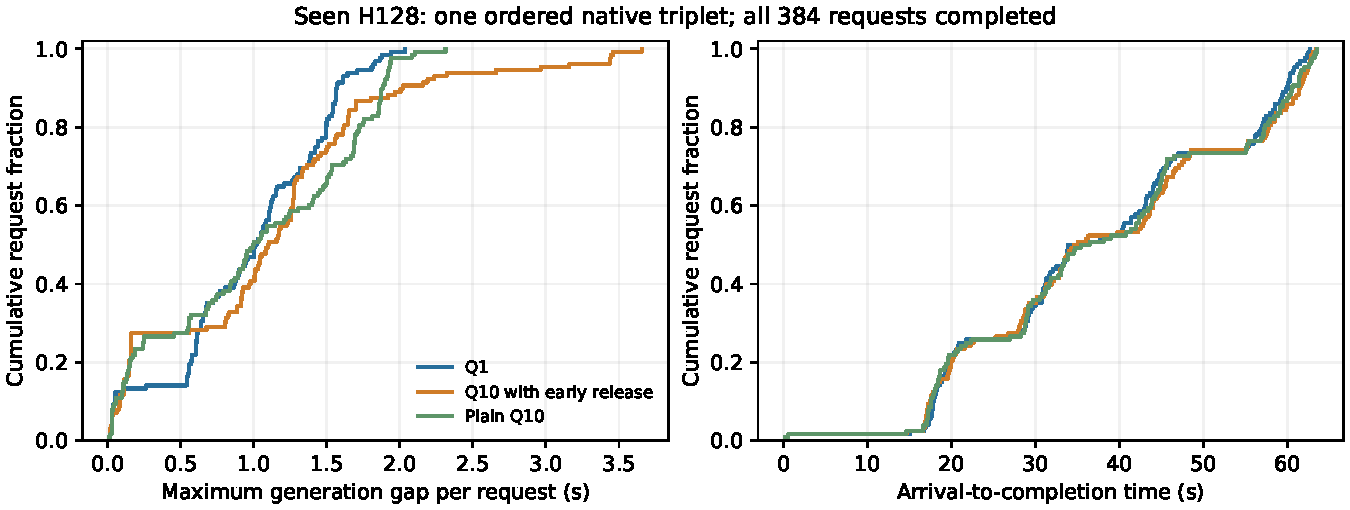
\includegraphics[width=\linewidth]{../A_PROTECTION_YIELD_TRIPLET_FIGURE_R01_20261001.pdf}
\caption{Complete-request distributions in the ordered Q1, conditional-release Q10, plain-Q10 exploration. Each arm includes all 128 requests. Output sequences differ across arms; this is a policy-level observation on seen data, not an equal-work or single-action causal comparison.}
\label{fig:yieldtriplet}
\end{figure}

\section{One Follow-up After Primary Recovery}
The earlier fit-first rule could replace an unfunded oldest recovery target and repeatedly bypass it. We instead test one bounded follow-up after the original target has already returned its first new output. A read-only reconstruction of the earlier H1 diagnostic found 93 of 267 forced-commit states with numerical capacity for both the original target and another paused request. At the original target's first output, 85 alternatives still numerically fit and 49 also met the existing 30-step absence requirement. These states motivate a live check; they do not establish transfer, ownership, or slot eligibility \cite{spareopportunity}.

The new arm retains capacity-qualified victim selection and Q1. Only the first output of an ordinary forced recovery can open one follow-up opportunity. If the actual PREEMPTED queue head needs more blocks than are free, the adapter considers the longest-absent eligible paused follower whose full history currently fits. It requires known zero in-flight reservations, no registered or pending transfer work, legal native slots and ownership, and pure decode. It uses the existing single-target native admission and first-output protection. It does not force another victim, and a follow-up's own output cannot trigger another follow-up. These restrictions bound actions per primary recovery, not request waiting time; a request can still be bypassed by several different primary recoveries. Unknown state retains the ordinary Q1 path. This is a stronger simple reference, without a novelty or starvation-bound claim \cite{sparepair}.

\begin{table}[t]
\centering
\caption{First ordered spare-follow-up pair on seen H128. Both arms completed all 128 arrivals.}
\label{tab:sparepair}
\begin{tabular}{lrr}
\toprule
Metric & Q1, off & Q1 + follow-up, on \\
\midrule
Actual output tokens & 125,069 & 124,444 \\
Output tokens/s & 1,435.944 & 1,425.151 \\
Mean flow (s) & 38.066 & 38.091 \\
Request gap median (s) & 1.137 & 0.888 \\
Request gap p95 (s) & 2.069 & 1.504 \\
Maximum gap (s) & 2.967 & 1.566 \\
TTFT p90 (s) & 40.291 & 39.848 \\
Actual preemptions & 357 & 400 \\
Forced rotations & 313 & 335 \\
One--two-output preemption pairs & 20 & 33 \\
Follow-up admissions & 0 & 24 \\
\bottomrule
\end{tabular}
\end{table}

The first off/on block completed 256/256 requests in total. All 24 choices had a same-step native asynchronous admission, a later new output, and completion. Each followed a recorded actual primary output, originated from an ordinary recovery, and had no actual same-step preemption. Admission-to-output median and maximum were 48.0 and 50.9 milliseconds. The candidate retained 99.248\% of Q1 output rate and 100.066\% of mean flow while reducing maximum gap from 2.967 to 1.566 seconds, passing all prespecified exploratory conditions. Across all requests, 82 maximum gaps improved and 46 worsened; flow improved for 57 and worsened for 71. Fourteen of the fixed twenty goodput points increased and six decreased. Sixty output sequences and one stop reason differed. This is one seen-input policy comparison, not equal-work acceleration or an action-level causal estimate \cite{sparepair}.

In all 24 action instances the bypassed queue head was the original primary victim. Its next output after the choice had median 0.545 seconds and maximum 1.414 seconds; all completed. These 24 instances involved 19 distinct requests, of which five had a larger full-request gap and twelve had larger flow than their off-arm counterpart. Eight actions also passed a distinct longest-absent waiter. The largest individual flow regression was 21.147 seconds for request 0017843, with 1,024 outputs and length termination in both arms. Its TTFT already differed by 17.538 seconds before its two appearances as a primary target with a follow-up. Consequently, that complete-request loss cannot be attributed to those two local actions alone. Actor sets are selected after actions and their costs overlap \cite{sparepeer}.

The candidate increased total preemptions and the count of short post-recovery service intervals. Seven complete printed transfer intervals per arm recorded off/on store 39.393/41.744 GB and load 117.480/126.490 GB. Boundary transfers remain unmeasured by these printed sums, and their CUDA event times are not request-visible delays. Both formal intervals had zero final-mtime cache-write records, without establishing zero compilation. The positive gap result therefore does not imply lower transfer volume or fewer preemptions \cite{sparetransfers,sparepair}.

\begin{figure}[t]
\centering
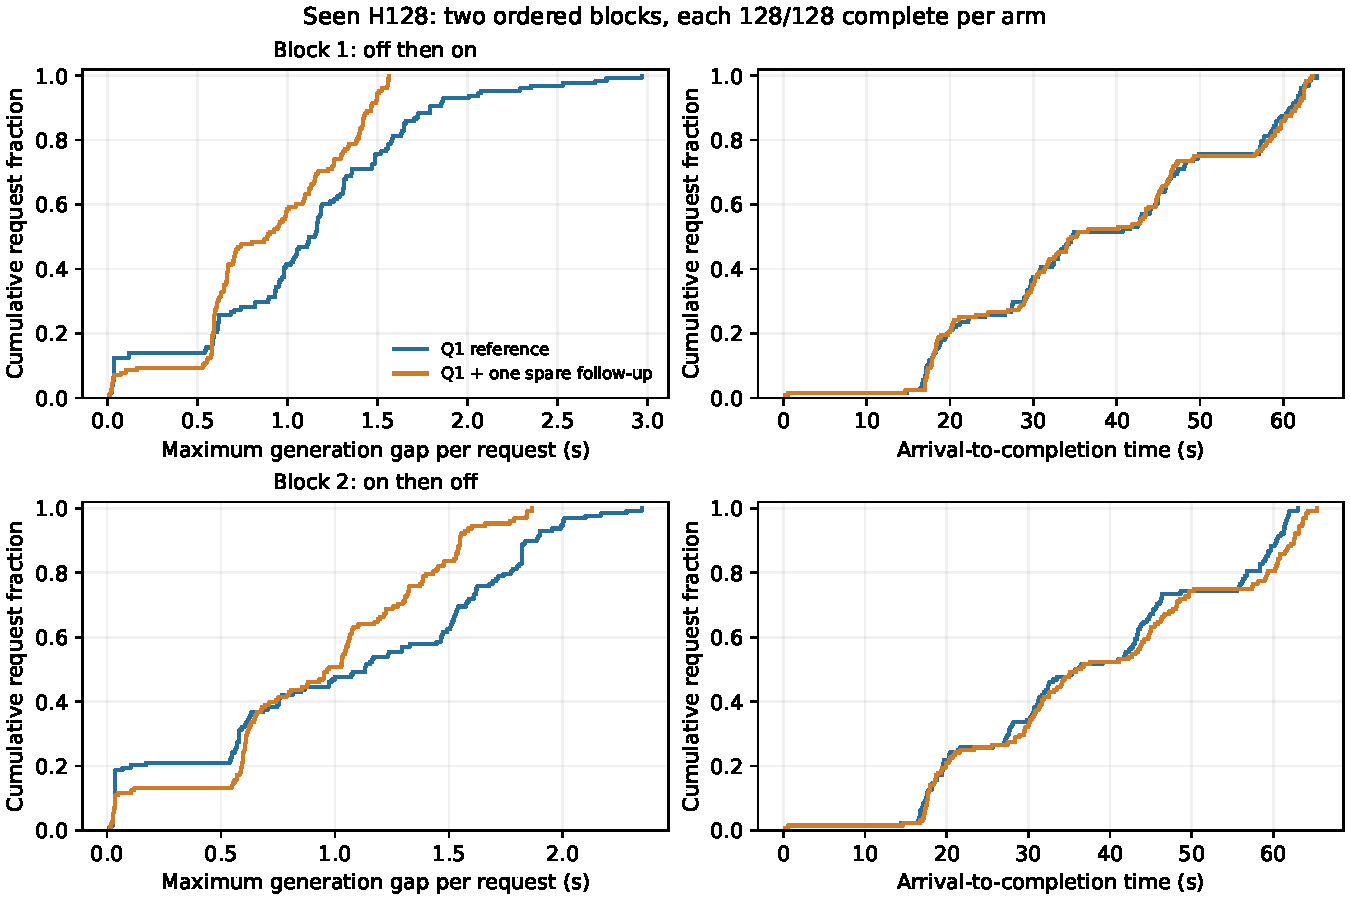
\includegraphics[width=\linewidth]{../A_SPARE_FOLLOWUP_TWO_PAIRS_FIGURE_R01_20261001.pdf}
\caption{All 128 requests per arm in each spare-follow-up block, equally weighted and kept separate. Gap improvements coexist with individual regressions and larger completion costs in the reverse block.}
\label{fig:sparepair}
\end{figure}

\paragraph{Reverse-order replication.}
The second block ran on/off with identical policy bytes, inputs, parameters, cache source, and criteria; all 256 requests completed. Its off/on rates were 1,431.062/1,405.295 tokens/s, mean flow 37.673/38.743 seconds, p95 request gaps 1.996/1.639 seconds, and maximum gaps 2.346/1.866 seconds. Thus rate was 98.199\% and mean flow 102.842\% of the off reference. All 24 follow-ups again had native admission, new output, and completion after primary output, with no same-step extra preemption or recursive origin. Both blocks independently passed every original criterion, without pooled cancellation. The two retained blocks are a replication on seen inputs, not a variance estimate or untouched-input confirmation \cite{sparetwopairs}.

In the reverse block, 71 request gaps improved and 57 worsened, while flow improved for only 24 and worsened for 104; TTFT improved for 15 and worsened for 113. Eight goodput points increased and twelve decreased. Both arms returned 124,453 tokens with 121 length and seven stop endings, but 57 sequences differed. Off/on preemptions were 326/379, forced rotations 283/320, and one--two-output preemption pairs 17/35. The bypassed victims' next-output time had median 0.615 seconds and maximum 1.479 seconds. Among 18 distinct such heads, ten had worse full-request gaps and sixteen worse flow than their off counterpart. Request 0009935, for example, had gap 1.866 versus 0.561 seconds even though the cohort maximum improved. These are policy-trajectory outcomes, not losses attributable to an isolated follow-up \cite{sparetwopairs,sparepeerr02}.

\section{Frozen New-input Triplet}
After both seen-input blocks passed, we froze the policy, off/on/native execution order, eligibility rules, and original rate/flow/gap criteria before selecting new inputs. The reader used the same pinned WikiText revision, a separately hashed Parquet representation, and the pinned OLMoE tokenizer. It selected the first 128 source-order complete articles after excluding all rows below 21,131 and known materialized A input identities and content. Fixed full-token eligibility was 256--3,072; selected lengths were 444--3,066 and the last article ended at row 37,347. All 192 previously materialized full G/H articles matched in rows, text, and tokens between the new reader and existing records. Partial warm-up articles were excluded conservatively by the old row prefix. This establishes freshness relative to that documented selection coverage, not globally unseen text. Arrivals remained spaced by 0.2 seconds with a 1,024-output cap and natural EOS. Serving-policy Python was unchanged; only inputs and the native-reference launch branch changed \cite{sparefresh}.

\begin{table}[t]
\centering\small
\caption{One frozen new-input episode, 128/128 complete per arm. The Q1 off arm is the prespecified budget reference. Native full saving is a separate system reference.}
\label{tab:sparefresh}
\begin{tabular}{lrrr}
\toprule
Metric & Q1 off & Q1 + follow-up & Native full \\
\midrule
Output tokens & 125,231 & 125,836 & 125,635 \\
Output rate (tokens/s) & 1,472.515 & 1,463.713 & 1,497.949 \\
Mean flow (s) & 39.216 & 39.524 & 35.977 \\
Median TTFT (s) & 14.293 & 15.021 & 21.661 \\
p90 TTFT (s) & 41.765 & 42.696 & 34.876 \\
Median request max gap (s) & 1.137 & 0.736 & 0.044 \\
p95 request max gap (s) & 2.062 & 1.670 & 7.499 \\
Maximum request gap (s) & 2.387 & 1.844 & 12.586 \\
Actual preemptions & 359 & 465 & 43 \\
Printed store (GB, partial) & 38.277 & 36.472 & 38.296 \\
Printed load (GB, partial) & 105.208 & 138.439 & 12.600 \\
\bottomrule
\end{tabular}
\end{table}

All 384 requests completed without failure or unfinished work. The on/off rate ratio was 99.402\% and mean-flow ratio 100.785\%, while maximum gap decreased by 22.754\%. All 18 follow-ups had a native asynchronous admission, subsequent new output, and completion. Actual primary output preceded every action; no follow-up recursively triggered another or introduced a same-step preemption. Admission-to-output median and maximum were 48.9 and 52.3 milliseconds. Thus all original acceptance conditions and native-reference completeness passed; no sample replacement or rescue run was used \cite{sparefresh}.

The complete-request costs remain material. Relative to off, on improved 88 request gaps and worsened 40, improved flow for 39 and worsened it for 89, and improved TTFT for 30 while worsening it for 98. Thirteen fixed goodput points increased and seven decreased. There were 62 different output sequences and three different stop reasons; off ended 121 requests by length and seven by stop, versus 122 and six on. Preemptions increased from 359 to 465, forced rotations from 322 to 403, and one--two-output preemption pairs from 13 to 35. Each arm had zero formal-interval cache writes by final-mtime accounting, with 32 initialization files written; this is not proof of zero compilation \cite{sparefresh}. Seven complete printed transfer intervals per arm recorded 105.208/138.439/12.600 GB of off/on/native loads and 38.277/36.472/38.296 GB of stores. The first possibly mixed interval and unprinted tail remain outside these sums. CUDA copy times do not measure request-visible delay; partial byte totals are retained separately from latency \cite{sparefreshtransfers}.

\begin{figure}[t]
\centering
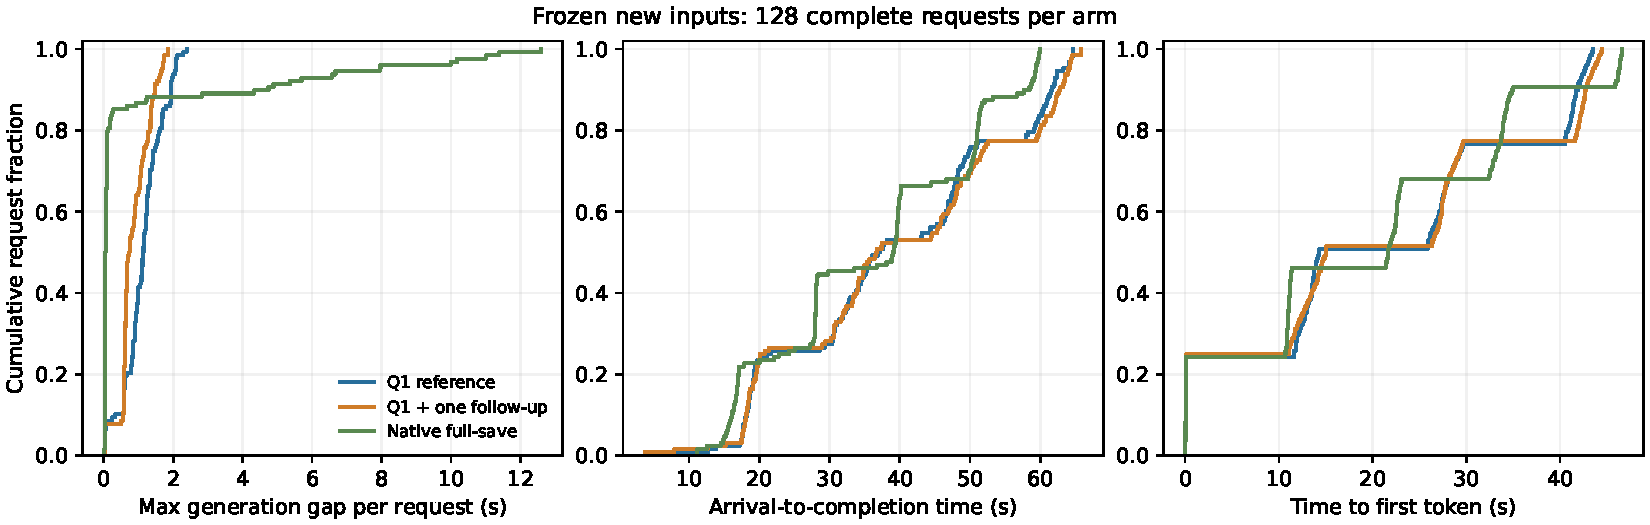
\includegraphics[width=\linewidth]{../A_SPARE_FOLLOWUP_FRESH_FIGURE_R01_20261001.pdf}
\caption{All requests in the frozen new-input triplet. Native full saving has a smaller median gap and mean flow but a longer gap tail. The follow-up improves the Q1 gap distribution while retaining individual and aggregate completion costs.}
\label{fig:sparefresh}
\end{figure}

All 18 bypassed heads were the original victims, covering sixteen distinct requests. Their next output after the choice had median 0.581 seconds and maximum 1.108 seconds; ten had worse full-request flow and two worse maximum gaps than off. Six distinct longest-absent waiters were also passed, all with worse flow. The largest individual gap regression was request 0022497: 0.626 to 1.736 seconds. It received a follow-up and new output, then was preempted later; 1.685 seconds preceded recorded admission and 49 milliseconds followed it. No follow-up occurred inside that longest gap. These observed trajectories locate a residual after limited Q1 service, without attributing the gap difference to the earlier action or reopening the already failed Q10 rule \cite{sparefreshpeer}.

Against native full saving, the follow-up achieved 97.714\% of output rate and 109.858\% of mean flow. It exceeded native goodput at twelve fixed points and fell below it at eight. Native saving and scheduling both differ, so this is a complete-system tradeoff rather than attribution to the follow-up alone. The off/on comparison retains the fixed backend and isolates the policy choice at the episode level. One new-input episode supports the declared narrow tradeoff, without establishing statistical significance, a hard gap bound, output quality, or an independent scheduling contribution \cite{sparefresh}.

\section{Ordinary Backfill as a Stronger Simple Control}
A positive comparison against Q1 alone does not establish that the primary-output trigger is necessary. The earlier fit-first experiment replaced a proposed forced recovery target, so it is not the same control. We therefore add ordinary eligible backfill: when no plan or protection is active, the actual PREEMPTED queue head does not fit, and the same native reservation, transfer, ownership, slot, full-history, and 30-step-age gates pass, choose the same longest-absent eligible follower. It retains Q1 first-output protection and adds no forced victim. It can act without a preceding regular-primary output, and may select another independently eligible follower after its own protection ends. Unknown state retains Q1. Only this trigger differs between the two backfill arms; neither is proposed as a new scheduling primitive \cite{waitercontrol}.

The original GPU was busy, so the complete frozen Q1/ordinary/primary-first block ran on the authorized backup RTX 5090 under its existing shared lock. Each cell received a private copy of the same completed 331-file, 81,577,847-byte cache from that machine. The three cells share policy package, input bytes, native backend, and resource budgets; they are compared within this block. The articles are now seen development inputs. We do not pool their timing with the preceding GPU, or claim a new confirmation episode \cite{waitercontrol}.

\begin{table}[t]
\centering\small
\caption{One same-GPU strong-control block. All 384 requests completed. Both candidates are judged separately against this block's Q1 reference.}
\label{tab:waitercontrol}
\begin{tabular}{lrrr}
\toprule
Metric & Q1 & Ordinary backfill & Primary-first \\
\midrule
Output tokens & 125,007 & 124,295 & 126,673 \\
Output rate (tokens/s) & 1,547.549 & 1,532.668 & 1,545.904 \\
Mean flow (s) & 36.606 & 36.412 & 36.932 \\
Median TTFT (s) & 13.489 & 13.812 & 12.643 \\
Median request max gap (s) & 1.141 & 0.575 & 1.011 \\
p95 request max gap (s) & 2.783 & 1.440 & 1.517 \\
Maximum request gap (s) & 3.407 & 1.894 & 1.711 \\
Actual preemptions & 348 & 496 & 433 \\
Forced rotations & 301 & 408 & 373 \\
One--two-output preemption pairs & 22 & 42 & 30 \\
Actual backfill chains & 0 & 44 & 19 \\
\bottomrule
\end{tabular}
\end{table}

Ordinary backfill achieved 99.038\% of Q1 output rate and 99.469\% of mean flow, with maximum gap decreasing from 3.407 to 1.894 seconds. The primary-first arm achieved 99.894\% of Q1 rate and 100.890\% of mean flow, with maximum gap 1.711 seconds. Both independently passed the original full-completion, real-action, rate, flow, and gap conditions. All 44 ordinary and 19 primary-first choices had native asynchronous admission, subsequent new output, and completion, without observed same-step preemption. Of the ordinary actions, 36 occurred outside a same-step regular-primary output release, demonstrating an actual trigger difference. Admission-to-output medians were 45.6 and 46.1 milliseconds; release-step associations are observations, not causal ancestry \cite{waitercontrol}.

Ordinary versus Q1 improved 105 request gaps and worsened 23; primary-first versus Q1 improved 76 and worsened 52. Directly against ordinary, primary-first improved only 33 request gaps and worsened 95, although its cohort maximum was 0.182 seconds lower. Its output rate was 100.864\% of ordinary and mean flow 101.429\%. Ordinary had higher goodput at all twenty prespecified points. This rate is the count of qualifying requests divided by each arm's own capture duration, 81.097 versus 81.941 seconds. Ordinary qualified more requests at sixteen points; at the four points with TTFT at most 40 seconds and gap bounds of 2--12 seconds, it qualified 122 rather than 123. Its rate advantage at those four points was only 0.003289 requests/s, due to the shorter duration. Thus the primary-output trigger is not needed to meet this block's declared objective, while the lower single maximum remains a descriptive tradeoff. Neither policy dominates every metric. The ordinary/Q1, primary-first/Q1, and primary-first/ordinary comparisons had 60/57/66 changed output sequences and 3/4/3 changed stop reasons; these are not equal-work speedups \cite{waitercontrol}.

\begin{figure}[t]
\centering
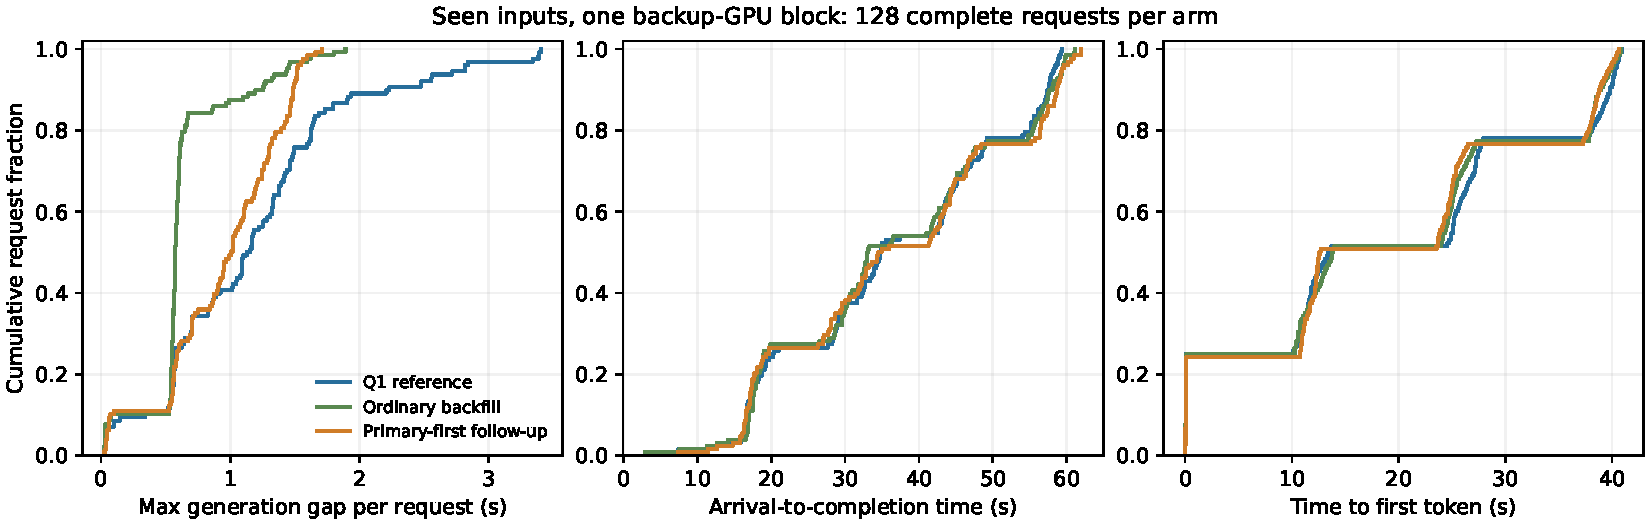
\includegraphics[width=\linewidth]{../A_WAITER_BACKFILL_TRIPLET_FIGURE_R01_20261001.pdf}
\caption{Full-request distributions for the strong simple control. Ordinary backfill improves most gaps and all fixed goodput points relative to primary-first, while primary-first retains a lower single worst gap.}
\label{fig:waitercontrol}
\end{figure}

Costs also fall on bypassed requests. Ordinary backfill bypassed the actual queue head 44 times across 25 requests, including 14 repeatedly bypassed heads; primary-first had 19 bypasses across 18 requests. Ordinary's worst-gap request had a 1.894-second gap after native preemption and was skipped as the oldest waiter twice during that gap. Its sparse trace does not expose the eventual admission time. The primary-first worst-gap request spent 1.664 seconds from native preemption to recorded asynchronous admission, then 46.5 milliseconds to output. These are actual trajectory locations, not attribution of a whole gap to an individual backfill choice \cite{waiteractors}.

The seven complete printed transfer intervals per arm recorded Q1/ordinary/primary-first stores of 39.137/39.695/40.181 GB and loads of 111.734/164.098/142.684 GB. Corresponding CUDA load-event sums were 2.021/2.967/2.578 seconds; these are not request waiting times. The first potentially warm-up-contaminated interval is excluded and the unprinted tail is unknown. Ordinary backfill therefore also carries a larger observed transfer and preemption cost than primary-first; neither partial counters nor endpoint caches are a full-episode accounting substitute \cite{waitercontrol}.

Formal-interval final-mtime cache writes numbered 32/16/32 files (1,477,946/655,329/1,477,946 bytes) in Q1/ordinary/primary-first. Each initialized 32 further files and had zero warm-up writes. Equal private seed caches do not establish zero compilation or identical overhead. All 110 raw files and all three outcomes were retained. This one ordered development block strengthens the simple reference and narrows the claim; it does not establish statistical significance or resolve the independent-method gap \cite{waitercontrol}.

\begin{figure}[t]
\centering
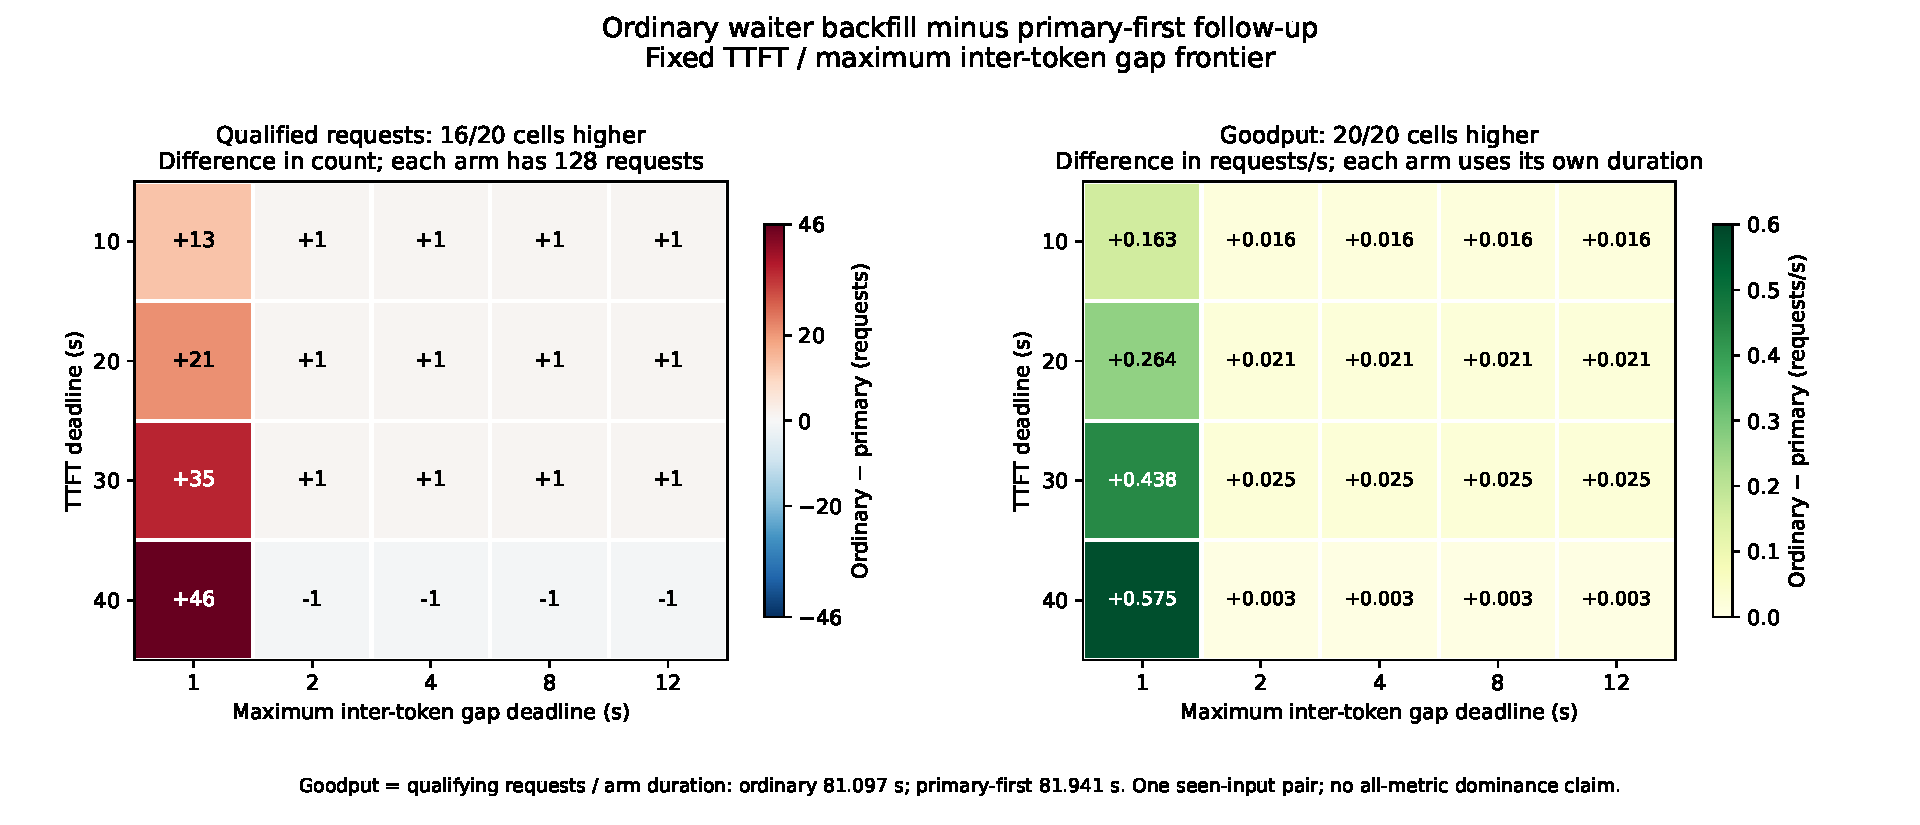
\includegraphics[width=\linewidth]{../A_WAITER_BACKFILL_FRONTIER_DELTA_R01_20261001.pdf}
\caption{Ordinary minus primary-first at all twenty fixed points. Qualifying counts improve at sixteen points, whereas rates improve at all twenty because each rate uses its own episode duration. This is not dominance over every service metric.}
\label{fig:waiterfrontier}
\end{figure}

\section{Native Full Saving Without Forced Rotations}
The preceding ordinary-backfill arm retained proactive capacity-qualified rotations. To separate the simple backfill action from those rotations, we run one further ordered pair on the original GPU: unchanged native full saving, then native full saving with ordinary eligible backfill and Q1 first-output protection. The second arm disables the entire proactive proposal/prepare branch and asserts that no forced rotation was applied. Both arms retain the native full-save calculation; the reference installs no scheduler adapter. The original native reservation, ownership, transfer, slot, age, and full-history gates remain. These are seen development articles and a simple-control extension, not a new method or another fresh confirmation \cite{nativeonly}.

\begin{table}[t]
\centering\small
\caption{Same native full-save backend, one ordered pair. Both cells completed all 128 arrivals. The candidate failed the fixed native-relative rate and mean-flow budgets.}
\label{tab:nativeonly}
\begin{tabular}{lrr}
\toprule
Metric & Native reference & With ordinary backfill \\
\midrule
Output tokens & 126,660 & 124,956 \\
Output rate (tokens/s) & 1,511.666 & 1,422.598 \\
Mean flow (s) & 35.924 & 37.801 \\
Median TTFT (s) & 21.578 & 23.790 \\
Median request max gap (s) & 0.042 & 0.051 \\
p95 request max gap (s) & 8.725 & 3.740 \\
Maximum request gap (s) & 13.101 & 11.844 \\
Actual native preemptions & 51 & 64 \\
Adapter forced rotations & N/A & 0 \\
Actual backfill chains & 0 & 23 \\
\bottomrule
\end{tabular}
\end{table}

All 23 choices had native asynchronous admission, subsequent new output, and final completion, with no same-step observed preemption. Admission-to-output median/p95/maximum were 50.0/62.0/67.0 milliseconds. No regular-primary release exists in this arm, confirming that these actions do not rely on proactive rotations. The candidate retained 94.108\% of native output rate, below the fixed 97\% floor, and raised mean flow to 105.225\%, above the 105\% ceiling. Its lower worst gap therefore does not satisfy the joint criterion. At request level, gaps improved for 69 and worsened for 59; flow improved for nine and worsened for 119; TTFT improved for 18 and worsened for 110. Goodput improved at five points and worsened at fifteen. There were 63 changed output sequences and two changed stop reasons; native had 123 length/five stop endings, versus 121/seven. This is not equal-work acceleration \cite{nativeonly}.

The 23 actions recovered 11 distinct targets, ten of which were later natively preempted after their first new output. They bypassed 14 distinct queue heads, four more than once. The candidate's longest-gap request, \texttt{0035191}, had no output from 62.068 to 73.912 seconds after an actual preemption at 62.070 seconds; it appeared once as an unfunded head and three times as the bypassed oldest waiter. Its native admission time is unrecorded, so this interval cannot be assigned entirely to queueing or any one backfill choice \cite{nativeonlypeer}.

\begin{figure}[t]
\centering
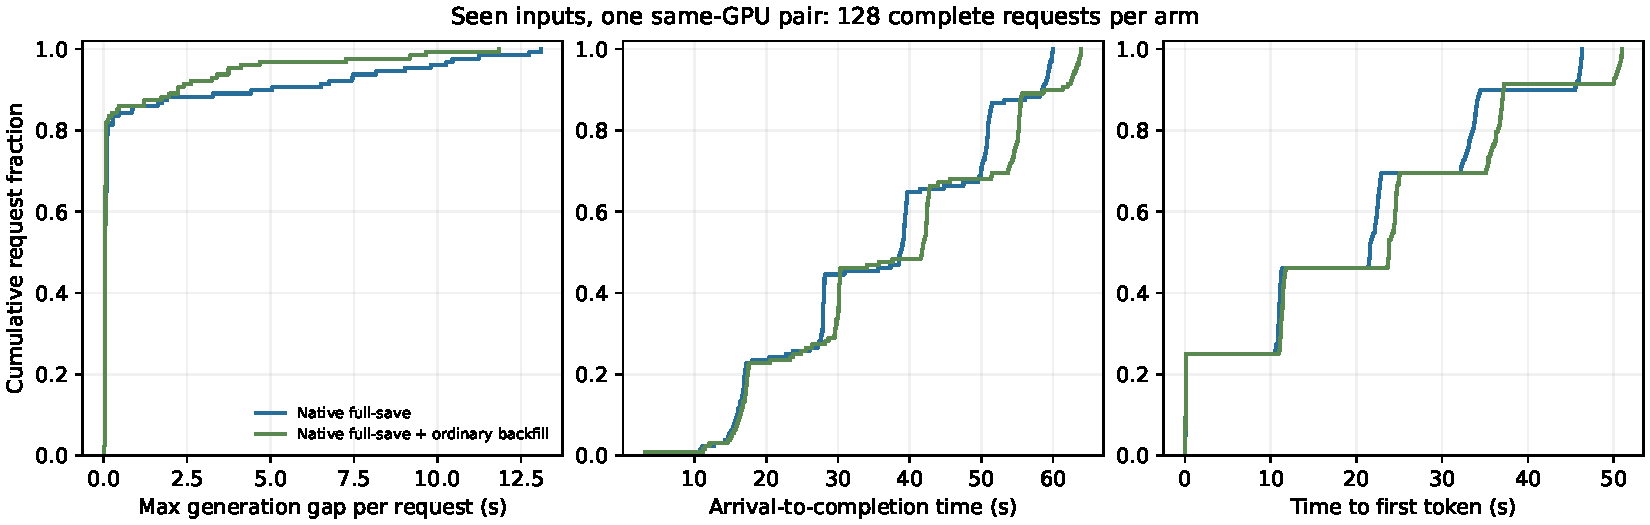
\includegraphics[width=\linewidth]{../A_NATIVE_BACKFILL_ONLY_FIGURE_R01_20261001.pdf}
\caption{Every request in the native full-save pair. Ordinary backfill reduces the large-gap tail but worsens completion and first-token latency for most requests.}
\label{fig:nativeonly}
\end{figure}

Both cells received separate copies of the same 525-file cache. Each initialized 32 files; final-mtime accounting found zero warm-up and formal-interval writes, which does not prove zero compilation. Seven complete printed intervals recorded native/candidate stores of 38.174/37.482 GB and loads of 15.066/17.329 GB; CUDA load-event sums were 0.294/0.330 seconds. The first possibly mixed interval is excluded and the unprinted tail remains unknown. These sums are not full-episode byte totals or request waiting times. This single ordered pair fails the exact fixed joint criterion for this ordinary-only formulation; it does not exclude other legal recovery schedules or establish statistical stability \cite{nativeonly,nativeonlytransfers}.

A separate instrumented ordinary-only diagnostic completed all 128 requests and observed twenty native-admitted backfill chains with no adapter-forced rotation. Its four disjoint adapter segments were captured at formal measurement end; native scheduler execution, GPU work, and asynchronous transfers are outside their timers. In this diagnostic, the segments summed to 2.721 seconds of host wall time (2.655 seconds of thread CPU), or 3.271\% of its own 83.160-second measurement interval. Most measured adapter time was in the per-step \texttt{begin} segment. These timed measurements locate host work within this one run; instrumentation adds overhead, and the result is not an incremental-delay estimate for the earlier pair or a cross-GPU service comparison \cite{nativeonlycpu}.

\begin{table}[t]
\centering\small
\caption{Adapter host timing in one instrumented native full-save ordinary-backfill diagnostic. Disjoint segment totals at formal measurement end; the sum of calls counts each segment invocation.}
\label{tab:nativeonlycpu}
\begin{tabular}{lrrr}
\toprule
Segment & Calls & Wall (s) & Thread CPU (s) \\
\midrule
\texttt{begin} & 5,479 & 2.534779 & 2.530850 \\
\texttt{hold} & 126,737 & 0.130115 & 0.085890 \\
\texttt{schedule\_pre} & 5,479 & 0.022328 & 0.009224 \\
\texttt{schedule\_post} & 5,479 & 0.033352 & 0.029095 \\
\midrule
Sum & 143,174 & 2.720574 & 2.655059 \\
\bottomrule
\end{tabular}
\end{table}

\subsection{Removing Unused Running-State Construction}
The diagnostic motivates a narrow implementation change. With forced rotations and detailed diagnostics disabled, the adapter still constructed a physical-block-checked view of every running request at every \texttt{begin} call, even when no active branch consumed it. The revised version constructs these views only for forced selection, diagnostic snapshots, initial closed-cohort activation, or a pending commit. Ordinary admission and protected-target checks retain their ownership, transfer, and capacity gates. This can defer detection of invalid ownership during an inactive step, so it is not an equivalence claim over all exceptional states. It changes no scheduling threshold or recovery objective.

One original-then-revised pair on the same backup GPU used identical host timers and separate copies of the same 427-file cache. Both cells completed all 128 requests and retained nineteen/twenty-seven native asynchronous admission--output--completion chains, with zero adapter-forced rotations. Mean \texttt{begin} thread CPU fell from 736.98 to 113.57 microseconds per call (84.59\% lower), meeting the separately frozen implementation-cost target of at least halving it. Total measured adapter wall time fell from 4.326 to 0.999 seconds, or 4.738\% to 1.122\% of each arm's own formal interval. Post-request drain made zero calls in both cells \cite{nativelazy}.

\begin{table}[t]
\centering\small
\caption{One same-host implementation-cost pair with identical timers. These are two ordinary-backfill arms, not a native-without-adapter comparison.}
\label{tab:nativelazy}
\begin{tabular}{lrr}
\toprule
Metric & Original views & On-demand views \\
\midrule
\texttt{begin} calls & 5,472 & 5,396 \\
\texttt{begin} thread CPU (s) & 4.032773 & 0.612827 \\
All adapter thread CPU (s) & 4.224753 & 0.849117 \\
Output tokens & 126,626 & 127,483 \\
Output rate (tokens/s) & 1,387.713 & 1,432.461 \\
Mean flow (s) & 40.749 & 40.961 \\
Maximum request gap (s) & 11.690 & 11.731 \\
Native preemptions & 59 & 62 \\
\bottomrule
\end{tabular}
\end{table}

Output rate was 103.225\% of the original, and mean flow was 100.519\%, within this pair's 97\%/105\% service guardrails. Maximum gap did not improve. Request gaps improved for 77 and worsened for 51; flow improved for 53 and worsened for 75; TTFT improved for 26 and worsened for 102. Goodput improved at seven fixed points and worsened at thirteen. There were 68 changed output sequences and one changed stop reason; the output counts differ by 857 tokens. Both cells initialized 32 cache files and had zero formal-interval final-mtime writes. These observations support retaining the cheaper implementation for further work, while preserving its mixed service consequences. They do not establish equal-work speedup, a new recovery mechanism, or repair of the earlier native-relative efficiency failure. The next pair compares the optimized implementation without timers against a contemporaneous native reference \cite{nativelazy}.

\subsection{Qualification Without Diagnostic Timers}
We freeze the same on-demand-view implementation without any host timing hooks and run one ordinary-then-native pair on the backup GPU. The native arm installs no scheduler adapter. Both arms retain full native saving, the same 128 seen articles, and separate copies of the same cache. The original native-relative conditions remain fixed: at least 97\% output rate, at most 105\% mean flow, lower maximum gap, complete requests, and actual ordinary recovery without forced rotation. No seed or policy threshold changes \cite{nativelazyperf}.

\begin{table}[t]
\centering\small
\caption{Untimed optimized ordinary/native qualification. Execution order was ordinary first, then native; columns show the native reference first for readability. Both completed 128/128 requests.}
\label{tab:nativelazyperf}
\begin{tabular}{lrr}
\toprule
Metric & Native reference & Optimized ordinary \\
\midrule
Output tokens & 126,565 & 124,886 \\
Output rate (tokens/s) & 1,444.756 & 1,527.506 \\
Mean flow (s) & 37.827 & 33.688 \\
Median TTFT (s) & 21.619 & 20.140 \\
p95 request max gap (s) & 10.373 & 5.159 \\
Maximum request gap (s) & 14.927 & 12.916 \\
Actual native preemptions & 49 & 59 \\
Actual backfill chains & 0 & 17 \\
\bottomrule
\end{tabular}
\end{table}

All nine original conditions pass in this block. The optimized arm reaches 105.728\% of native output rate and 89.058\% of native mean flow. All seventeen choices have native asynchronous admission, later output, and completion; median admission-to-output is 46.7 milliseconds, with no same-step observed preemption and no forced rotation. Per-request gaps improve for 111 and worsen for seventeen, flow improves for 127 and worsens for one, and TTFT improves for 123 and worsens for five. All twenty fixed goodput rates are higher. However, 75 output sequences and two stop reasons differ, with 1,679 fewer output tokens in the candidate. This is not equal-work acceleration \cite{nativelazyperf}.

\begin{figure}[t]
\centering
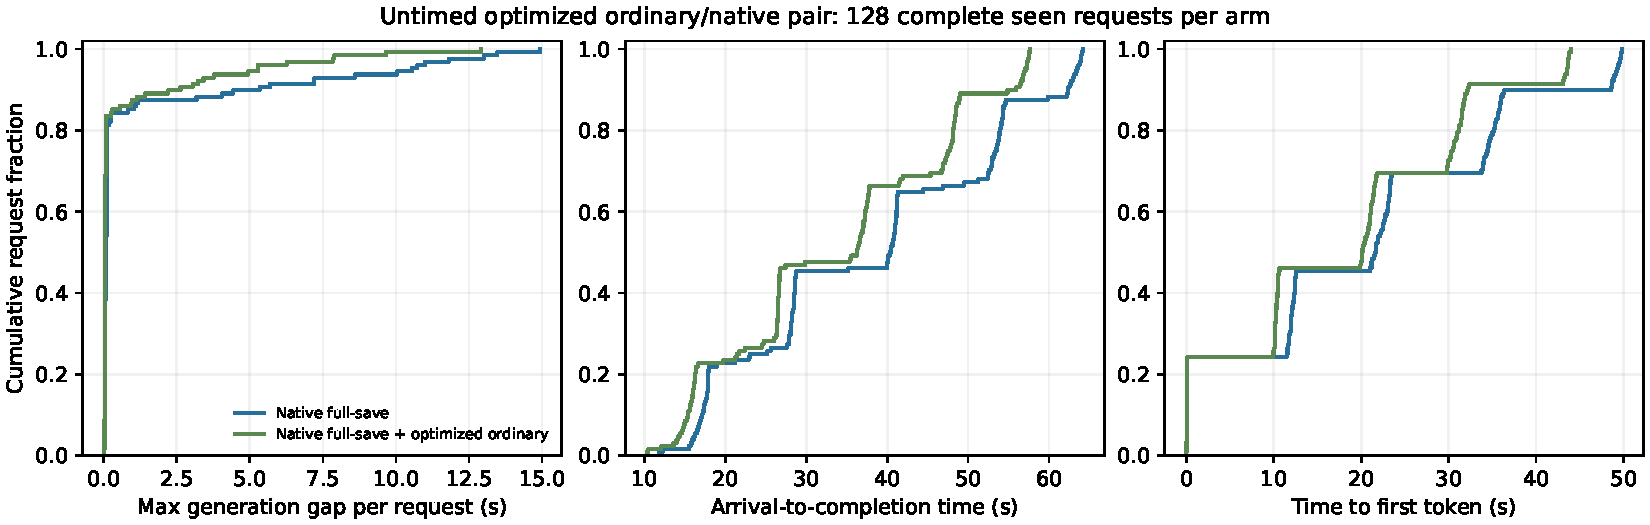
\includegraphics[width=\linewidth]{../A_NATIVE_BACKFILL_LAZY_PERF_FIGURE_R01_20261002.pdf}
\caption{All requests in the untimed optimized ordinary/native pair. Aggregate improvements coexist with seventeen individual gap regressions. This is one seen-input qualification block.}
\label{fig:nativelazyperf}
\end{figure}

The longest candidate gap belongs to request \texttt{0035191}: 12.916 seconds, versus 0.095 seconds for that request in the native arm. Yet its TTFT and completion improve by 19.989 and 7.360 seconds respectively. Its native admission time is absent from the sparse record; the interval cannot be assigned entirely to queueing or one backfill choice. Of ten distinct recovery targets, nine are later preempted again. The only completion regression is request \texttt{0027054}, by 0.201 seconds, alongside a 3.807-second worse gap. These observations preserve the individual tradeoff beneath the aggregate improvement \cite{nativelazyperfpeer}.

The two cells receive 459-file cache seeds, each initializes 32 files, and final-mtime accounting finds zero warm-up and formal writes. Native/candidate stores printed over seven complete intervals sum to 37.948/38.504 GB. Observed loads sum to 13.348/16.444 GB, but cover seven/six intervals respectively: one candidate interval has no printed load fields and is left missing. The potentially warm-up-mixed first print and unprinted tail are excluded. These partial records are not full-episode transfer totals or request waiting times \cite{nativelazyperfcost}. The earlier original-implementation failure remains valid in its original block. Neither that cross-host contrast nor this one reversed-order qualification identifies the entire service difference as a CPU effect. The result qualifies a stronger simple implementation; it is not a fresh-data or independent-method claim.

\section{Victim Choice at Actual KV Pressure}
The ordinary-only trace contains a concrete short-service residual: sixteen of seventeen backfill actions are followed by another actual native preemption; eleven produce at most sixteen new outputs between selection and that first re-preemption, with median thirteen. Only two reconstructed endpoints are exactly at a KV-page boundary, and one action produces 511 outputs. We therefore do not equate re-preemption with one-token thrashing or a target's own page-boundary failure \cite{residencyshort}.

The pinned FCFS scheduler appends a recovered request to the running list but pops its tail on allocation failure. We test a minimal action at that failure, using only the not-yet-processed running suffix so no earlier token assignment must be undone. All arms retain the same ordinary backfill, native full saving, and one-output admission protection. The controls select the native tail or the latest original arrival in that same suffix. The candidate chooses the largest
\[
 \rho_i=\frac{o_i-o_i^{\mathrm{admit}}}{b_i},
\]
where $o_i^{\mathrm{admit}}$ is recorded at this residence's actual native running admission, after an asynchronous load when one occurs, and $b_i>0$ is the current unshared physical KV-block count. This is a live service-density heuristic, not a measured transfer-cost model. An unknown or mixed suffix uses the native tail; ties choose the later index. No additional waiting hold or proactive preemption is introduced. The same admission accounting and decision records run in every arm.

\begin{table}[t]
\centering\small
\caption{One tail--arrival--density native triplet on the same seen 128 requests. All complete, with zero failures and zero adapter-forced rotations.}
\label{tab:residency}
\begin{tabular}{lrrr}
\toprule
Metric & Tail & Arrival & Residence density \\
\midrule
Output tokens & 125,722 & 125,971 & 125,838 \\
Output rate (tokens/s) & 1,571.383 & 1,568.270 & 1,554.088 \\
Mean flow (s) & 33.910 & 33.740 & 34.062 \\
Median TTFT (s) & 20.237 & 20.025 & 21.936 \\
p90 request max gap (s) & 2.250 & 1.672 & 2.730 \\
p95 request max gap (s) & 5.111 & 3.225 & 3.363 \\
Maximum request gap (s) & 12.172 & 8.415 & 6.222 \\
Actual native preemptions & 59 & 64 & 81 \\
Victim choices differing from tail & 0 & 10 & 76 \\
Backfill output/completion chains & 17 & 27 & 32 \\
\bottomrule
\end{tabular}
\end{table}

The density arm satisfies the predefined maximum-gap condition and 97\% rate/105\% mean-flow budgets against both controls. Its rate is 98.899\% of tail and 99.096\% of arrival; mean flow is 100.449\% and 100.954\%, respectively. All 204 victim decisions map to actual same-step native preemptions, including all 76 changed density choices. However, arrival has better p90 and p95 gaps, and density improves only 54 requests' maximum gaps while worsening 74. Relative to arrival it improves 29 completion times and worsens 99; TTFT improves for 32 and worsens for 96. Goodput is higher at seven fixed points and lower at thirteen. This is a constrained worst-gap benefit, not complete-request dominance \cite{residencyvictim}.

\begin{figure}[t]
\centering
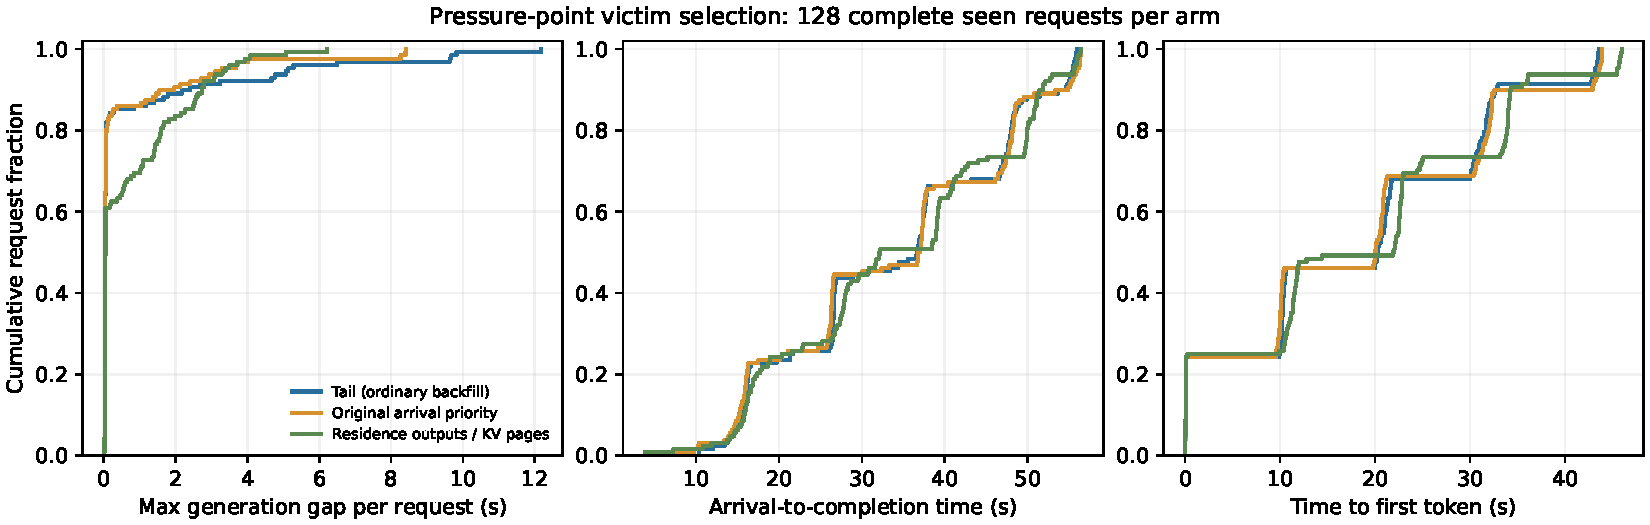
\includegraphics[width=\linewidth]{../A_NATIVE_RESIDENCY_VICTIM_FIGURE_R01_20261002.pdf}
\caption{All 128 requests in each victim-selection arm. Residence density shortens the cohort's longest gap while moving more requests into intermediate pauses.}
\end{figure}

Among qualified victim choices, the selected residence has produced a median 35/36/360.5 new outputs in tail/arrival/density; at most sixteen outputs occur in 17/57, 24/63, and 1/78 choices. These summaries include initial residences, not just restored requests. Density selects the currently allocation-failed request 31 times, versus five and one in the controls, and increases total preemptions. It therefore redistributes service rather than establishing reduced swapping. Output sequences differ for 63/65/59 requests in the three pairwise comparisons; each comparison changes two stop identities although all arms end with 122 length and six natural-stop completions. This is not an equal-work comparison.

Seven observed store-counter intervals sum to 38.766, 38.736, and 38.483 GB. Observed loads sum to 15.886, 17.031, and 18.478 GB, over six/six/seven intervals; missing last load fields in the two controls are not imputed as zero. These prints exclude the first possibly warm-up-mixed interval and any unprinted boundary work, and are not full-episode transfer or exposed-delay totals \cite{residencycost}. The three engines use separate copies of the same 491-file cache seed.

Joining each selected victim to its most recent native running admission separates restored residences from initial admission. Restored victims have produced a median 19, 35.5, and 311 new outputs in tail, arrival, and density; at most sixteen new outputs occur in 15/34, 12/38, and 1/30 restored epochs. These are selected-victim distributions, not guarantees for every restored request. The sparse trace does not contain a complete scheduled-token map, so exact zero-token scheduler steps remain unknown \cite{residencyepochs}.

\subsection{Separating Residence Reset and KV Normalization}
A second three-engine block compares the complete rule against residence outputs alone and lifetime outputs divided by current KV blocks. The candidate runs first; all three use the same seen requests and identical eligibility and fallback rules. This whole block runs on the primary GPU, whereas Table~\ref{tab:residency} ran on the backup; comparisons below stay within the block. All 128 requests complete in every arm, with zero adapter-forced rotations. Every victim decision joins to an actual native preemption \cite{residencyablation}.

\begin{table}[t]
\centering\small
\caption{Within-block factor ablation. Removing either factor does not cover the complete rule's joint maximum-gap and efficiency result.}
\label{tab:residencyablation}
\begin{tabular}{lrrr}
\toprule
Metric & Full density & Residence outputs & Lifetime density \\
\midrule
Output tokens & 125,911 & 127,483 & 125,808 \\
Output rate (tokens/s) & 1,498.711 & 1,475.048 & 1,468.987 \\
Mean flow (s) & 36.098 & 37.270 & 36.606 \\
Median TTFT (s) & 23.569 & 23.050 & 23.432 \\
p90 request max gap (s) & 3.111 & 2.683 & 3.330 \\
p95 request max gap (s) & 3.573 & 4.769 & 3.915 \\
Maximum request gap (s) & 5.020 & 8.533 & 9.081 \\
Actual native preemptions & 89 & 58 & 103 \\
Changed victim choices & 83 & 53 & 69 \\
\bottomrule
\end{tabular}
\end{table}

The complete rule has 1.604\% and 2.023\% higher actual output rate than the two ablations, with mean flow 3.145\% and 1.388\% lower. Its maximum gap is 41.164\% and 44.714\% lower. Both comparisons meet the fixed 97\% rate and 105\% flow conditions. However, residence outputs alone retains better median TTFT and p90 gap. Full density improves/worsens individual gaps for 70/58 requests against residence outputs and 74/54 against lifetime density; goodput is higher/lower at 12/8 and 11/9 fixed points. Output sequences differ for 55 and 60 requests, respectively, with two stop-identity differences in each comparison. This supports retaining both factors for the next frozen-input check, but one independently evolving block neither identifies their same-state causal effects nor establishes novelty or repeatability.

\subsection{New-Input Counterexample}
Both opposite-order confirmation blocks were frozen before their first GPU output. The next 128 source-ordered complete articles occupy rows 37,452--54,660 of the same pinned dataset, with full lengths 500--3,062 tokens, unchanged 0.2-second arrivals, and the same natural-EOS cap. Selection excludes the previous A inputs and validates 320 earlier complete articles by source text and tokenizer identity. This is new input relative to that known A inventory, not a claim of globally unseen data.

The first block runs density, arrival, and tail. All requests complete and every changed victim choice reaches an actual native preemption, but the candidate fails the fixed lower-maximum-gap condition against tail (Table~\ref{tab:residencyfresh}). Density has higher goodput than tail at only two fixed points and lower goodput at eighteen. Against arrival the split is eight higher and twelve lower. Output sequences differ for 68 requests against tail and 63 against arrival, with one and zero stop-identity differences \cite{residencyfreshb1}.

\begin{table}[t]
\centering\small
\caption{First frozen new-input block. The residence-density candidate fails the tail-relative maximum-gap objective.}
\label{tab:residencyfresh}
\begin{tabular}{lrrr}
\toprule
Metric & Density & Arrival & Tail \\
\midrule
Output tokens & 128,296 & 128,300 & 127,291 \\
Output rate (tokens/s) & 1,483.151 & 1,509.758 & 1,503.579 \\
Mean flow (s) & 37.933 & 37.640 & 36.999 \\
Median TTFT (s) & 24.135 & 22.388 & 22.087 \\
p90 request max gap (s) & 3.216 & 2.240 & 1.781 \\
Maximum request gap (s) & 10.071 & 11.573 & 8.391 \\
Actual native preemptions & 81 & 71 & 67 \\
\bottomrule
\end{tabular}
\end{table}

The reverse block runs tail, arrival, and density on the same frozen inputs. Again, all 384 arm-requests complete, changed victim choices join to actual native preemptions, and density passes both within-block rate and mean-flow budgets against each control. It fails the required maximum-gap comparison with tail: 9.034 versus 8.357 seconds, although it improves on arrival's 13.492 seconds (Table~\ref{tab:residencyfreshb2}). Density has higher/lower goodput than tail at 9/11 fixed points and than arrival at 3/17. Its individual gaps improve/worsen for 43/85 requests against tail; 64 output sequences and two stop identities differ. The original twelve-part criterion fails in each block, without pooling or selecting a favorable order. These serial blocks provide no variance estimate or same-state action effect \cite{residencyfreshb2,residencyfreshtwo}.

\begin{table}[t]
\centering\small
\caption{Reverse-order frozen new-input block. Density again fails the tail-relative maximum-gap objective.}
\label{tab:residencyfreshb2}
\begin{tabular}{lrrr}
\toprule
Metric & Tail & Arrival & Density \\
\midrule
Output tokens & 128,154 & 126,388 & 128,296 \\
Output rate (tokens/s) & 1,503.279 & 1,496.275 & 1,485.910 \\
Mean flow (s) & 37.744 & 36.521 & 38.049 \\
Median TTFT (s) & 22.656 & 22.135 & 24.230 \\
p90 request max gap (s) & 2.106 & 1.710 & 3.489 \\
Maximum request gap (s) & 8.357 & 13.492 & 9.034 \\
Actual native preemptions & 59 & 75 & 85 \\
\bottomrule
\end{tabular}
\end{table}

The density arm's worst request, article 0042224, pauses after output 588 of its 1,024-token cap. At scheduler step 1,567 it selects itself as victim with 496 residence outputs and 151 held blocks; the native tail has nine residence outputs and 87 blocks. The observed gap lasts from 23.105 to 33.177 seconds. Its first recorded asynchronous admission occurs about 10.024 seconds after preemption, followed by native running admission and a new output. In the tail arm, the same article's maximum gap is 1.715 seconds. These are different trajectories and do not isolate a same-state victim effect \cite{residencyfreshchain}.

A separate source-level consequence matters for interpreting the intervention. Native FCFS tail self-preemption implies that no later running requests remain, so the running scan exits. The density rule can instead select the allocation-failed current request while later requests remain, but inherits that exit. This occurs with 26 such self-preemptions in the first development density arm and 33 in the complete-score ablation. In the new-input worst case, thirty running successors remain. Their existence is not evidence that they could all receive tokens, and one missed scan cannot by itself explain the ten-second gap. A guarded continuation preserves the current index and re-enters the original successor checks; its actual service result follows \cite{residencyselfsuffix}.

\subsection{Guarded Self-Preemption Continuation}\label{sec:selfcontinue}
One ordered, same-input triplet compares native tail with the original break, density with the original break, and density with guarded continuation (Table~\ref{tab:selfcontinue}). All 128 requests complete in each arm, with no adapter-forced rotations. The guard applies at 29 self-preemptions: the original successor is visited, the source request schedules zero tokens, and joined successor records contain 319 same-call new outputs. Thus the mechanism executes, but the service criterion fails. Continuation meets the 97\% output-rate and 105\% mean-flow budgets against both break controls; its 10.750-second maximum gap exceeds 7.776 and 10.535 seconds, respectively. Goodput is lower at 14 of 20 fixed points against each control. Different natural outputs and stop identities limit causal interpretation; the ten-second tail is not removed \cite{residencycontinue}.

\begin{table}[t]
\centering\small
\caption{Same-input continuation pilot. Real successor work does not meet the fixed lower-maximum-gap condition.}
\label{tab:selfcontinue}
\begin{tabular}{lrrr}
\toprule
Metric & Tail break & Density break & Density continue \\
\midrule
Output tokens & 127,169 & 127,428 & 128,211 \\
Output rate (tokens/s) & 1,493.782 & 1,494.581 & 1,495.991 \\
Mean flow (s) & 37.515 & 37.285 & 37.650 \\
Maximum request gap (s) & 10.535 & 7.776 & 10.750 \\
Actual native preemptions & 61 & 85 & 75 \\
Natural stop completions & 4 & 4 & 3 \\
\bottomrule
\end{tabular}
\end{table}

\subsection{Pinned BidKV Score Control}
A separate triplet adapts the pinned official BidKV default score and tie order to our qualified, not-yet-scheduled running suffix, with native full saving and no proactive rotation. This is a restricted score control, not our method or a reproduction of the full BidKV scheduler. The pinned plugin's \texttt{pick\_victim} receives the running requests and policy without an allocation-failed-current parameter; that commit does not pin the host scheduler loop, so it cannot establish host prefix rollback or self-preemption continuation. We evaluate a separate current-request guard below only as native-loop adapter feasibility, not as a score contribution. All three arms complete 128 requests. BidKV with the original break changes 45 victim choices, all joined to actual native preemptions; against tail it meets the 97\% rate, 105\% mean-flow, and lower-maximum-gap conditions, with higher/lower goodput at 17/3 fixed points. In the separate continuation comparison, eight guards apply and the joined successors produce 89 same-call outputs. Continuation also meets those three service conditions against each break control, but its goodput is higher/lower at only 5/15 points against BidKV break and 11/9 against tail. Table~\ref{tab:bidkvscore} reports the complete cohort; changing natural outputs and one ordered seen-input block preclude a stability or same-state causal claim \cite{bidkvcode,bidkvresult}.

\begin{table}[t]
\centering\small
\caption{Pinned-score adaptation on one seen-input block. The score-only baseline and the separate continuation test meet their respective fixed conditions.}
\label{tab:bidkvscore}
\begin{tabular}{lrrrrr}
\toprule
Arm & Output tokens & Rate (tokens/s) & Mean flow (s) & Max gap (s) & Preemptions \\
\midrule
Tail break & 128,296 & 1,513.237 & 37.301 & 8.781 & 60 \\
BidKV break & 127,285 & 1,480.460 & 37.137 & 8.366 & 53 \\
BidKV continue & 128,296 & 1,485.885 & 37.722 & 7.181 & 59 \\
\bottomrule
\end{tabular}
\end{table}

In a second ordered, seen-input triplet with the same restricted score, the current-request guard changes four victim choices when the allocation-failed request would otherwise preempt itself. All four selected alternatives are actually preempted, the current request produces a token in the same engine call, and all four displaced requests later output and complete. All 128 requests finish in each arm, with no forced rotations. Table~\ref{tab:bidkvcurrentguard} shows that the guard meets the fixed 97\% rate, 105\% mean-flow, and lower-maximum-gap conditions against both break controls in this block. Its maximum gap is 7.764 seconds versus 9.861 and 8.382 seconds, but 37 and 40 individual request gaps worsen against the respective controls; fixed-point goodput improves at 14/20 and 19/20 points. The three arms generate different natural outputs: guard versus break/continue changes 64/63 sequences and 3/2 stop reasons. The canonical result retains all individual differences and displaced-victim interruptions, which cannot be interpreted as same-state causal costs. This guard is an adapter feasibility correction, not a new BidKV score or stable confirmation \cite{bidkvguardresult}.

\begin{table}[t]
\centering\small
\caption{Current-request guard on one ordered, seen-input block (128 completed requests per arm).}
\label{tab:bidkvcurrentguard}
\begin{tabular}{lrrrrr}
\toprule
Arm & Output tokens & Rate (tokens/s) & Mean flow (s) & Max gap (s) & Preemptions \\
\midrule
BidKV break & 127,348 & 1,491.631 & 37.157 & 9.861 & 51 \\
BidKV continue & 128,290 & 1,481.869 & 37.966 & 8.382 & 51 \\
BidKV current guard & 126,405 & 1,479.547 & 36.751 & 7.764 & 57 \\
\bottomrule
\end{tabular}
\end{table}

\subsection{Frozen Current-Guard Confirmation}
Before either new-input run, we fixed a disjoint cohort of 128 complete articles, the four arms, and both opposite execution orders. Each block had to satisfy all eighteen validity, mechanism, and service conditions independently. Table~\ref{tab:guardfresh} retains both blocks. Every arm completes all 128 requests with native full saving and zero forced rotations. The guard changes seven and five actual victim choices, respectively; every such current request produces an output in the same engine call, while every displaced victim later outputs and completes. These observations establish the local action but not its service benefit \cite{guardfreshtwo}.

\begin{table}[t]
\centering\small
\caption{Frozen current-guard confirmation. Orders are top to bottom within each block. Both blocks fail the original joint criterion. The tail anchor shares the ordinary native-full backend.}
\label{tab:guardfresh}
\begin{tabular}{llrrrr}
\toprule
Block & Arm & Output tokens & Rate (tokens/s) & Mean flow (s) & Max gap (s) \\
\midrule
1 & Tail break & 128,077 & 1,525.683 & 37.362 & 8.606 \\
1 & BidKV break & 127,141 & 1,494.663 & 37.367 & 5.997 \\
1 & BidKV continue & 127,071 & 1,491.013 & 37.405 & 8.654 \\
1 & Current guard & 127,109 & 1,492.263 & 37.257 & 6.870 \\
\midrule
2 & Current guard & 126,432 & 1,489.107 & 37.077 & 9.111 \\
2 & BidKV continue & 128,077 & 1,499.825 & 37.698 & 7.060 \\
2 & BidKV break & 130,061 & 1,503.199 & 38.458 & 9.549 \\
2 & Tail break & 129,314 & 1,537.946 & 38.095 & 8.850 \\
\bottomrule
\end{tabular}
\end{table}

Block 1 fails the lower-maximum-gap condition against BidKV break. Block 2 fails that condition against tail and BidKV continue, and its output rate is 96.824\% of tail, below the fixed 97\% budget. Goodput remains mixed: guard versus tail/break/continue improves at 16/11/15 of twenty points in block 1 and 19/20/13 in block 2. Output sequences differ for 52/55/58 and 63/60/58 requests, with 3/2/2 and 6/5/5 stop-reason differences. We retain those complete frontiers and do not replace the original objective with a favorable subset or pool the blocks.

The longest-gap request in block 1 is selected as an alternative victim by an ordinary score decision, outside the guard's current-request condition. At its first preemption it has produced 304 outputs and holds 206 pages; preemption, the next recorded running admission, and the next output occur at 26.459951, 33.313752, and 33.329497 seconds. Its 6.870386-second gap therefore exposes a limit of this guard's action coverage, without identifying the exact queue/load split or an alternative action's causal outcome \cite{guardfreshchain}. We stop expanding the unchanged guard. The remaining closest-baseline gap is whether score selection may evict already scheduled running requests: pinned native PRIORITY scheduling contains the required token, block, encoder, and index rollback, whereas our measured score adapters so far consider only the qualified unprocessed suffix. The full-running baseline below now qualifies this native rollback path; it is not a new scoring method.

In block 2, the longest-gap request is preempted a second time after only nine further outputs in its restored residence. The first recorded readmission and resumed output occur at 7.423875 and 7.440438 seconds; the second preemption is at 7.568664 seconds, followed by recorded readmission at 16.662584 and output at 16.678723 seconds. Both decisions select a request other than the allocation-failed current request, so neither triggers the guard. At the second decision, only suffix positions 26--28 are recorded as candidates; the earlier positions' identity, eligibility, and scores are unknown in these records. Thus this trace motivates measuring a larger candidate set, but cannot predict a prefix victim or its outcome. Held pages are also not an independently measured net-free-capacity increment \cite{guardfreshchainb2}.

\subsection{Full-Running BidKV Score Control}
One ordered, seen-input triplet extends the restricted pinned BidKV score from the unprocessed running suffix to qualified pure-decode requests throughout the running set. Tail, suffix, and full-running arms all complete 128 requests with native full saving and no forced rotations. All 17 full-running prefix choices join actual same-step native preemptions, verified token/block/index rollback, and omission of the victim from that call's output plan; none yields a same-call victim output, and all 17 victims later output and complete. Thus the stronger adapter passes its mechanism qualification. Table~\ref{tab:bidkvfullrunning} shows why it fails the separate service criterion: its 9.364-second maximum request gap exceeds both tail's 8.627 and suffix's 6.138 seconds, although its rate and mean flow satisfy the fixed 97\% and 105\% bounds against each. Full-running goodput improves/worsens at 7/13 fixed points versus tail and 9/11 versus suffix; 70/67 output sequences and 3/1 stop reasons differ. These complete-request comparisons are descriptive across different natural outputs, not equal-work or same-state effects. This is a qualified stronger baseline, neither a new method nor a full BidKV reproduction \cite{bidkvcode,bidkvfullrunning}.

\begin{table}[t]
\centering\small
\caption{Full-running pinned-score baseline on one ordered seen-input block (128 completed requests per arm). Mechanism qualification passes; the full-running arm fails the lower-maximum-gap condition against both controls.}
\label{tab:bidkvfullrunning}
\begin{tabular}{lrrrrr}
\toprule
Arm & Output tokens & Rate (tokens/s) & Mean flow (s) & Max gap (s) & Preemptions \\
\midrule
Tail break & 126,617 & 1,498.437 & 36.881 & 8.627 & 62 \\
BidKV suffix break & 128,154 & 1,479.641 & 37.690 & 6.138 & 46 \\
BidKV full break & 127,200 & 1,467.100 & 37.180 & 9.364 & 52 \\
\bottomrule
\end{tabular}
\end{table}

\subsection{Completion-Funded Prefix Deferral}
In one ordered, seen-input pilot, all three arms retain native full saving and complete 128 requests without forced rotations. At a native KV allocation failure, \emph{prefix work} defers the failed current request when an already scheduled pure-decode prefix can produce work; \emph{prefix finish} additionally requires a witness whose remaining hard output cap fits its currently owned physical KV capacity. The 9,091 work and 276 finish deferral events all join native plans and raw events, with later output and completion of the failed current request. Work involves 27 distinct witnesses and 115 failed current requests; finish involves eight and 47, respectively. None of these witnesses is re-preempted before completion \cite{completiongroups}. All 276 finish choices satisfy the cap check, but their eight distinct witnesses later terminate at the length cap, not natural EOS. These repeated events are mechanism evidence, not independent completion benefits \cite{completiondeferral}. Table~\ref{tab:completiondeferral} shows that work lowers the maximum gap relative to tail but misses both the 97\% rate floor (95.425\%) and 105\% mean-flow ceiling (106.739\%). Finish meets those budgets against both controls but has a higher maximum gap than both, so its separate service criterion fails. Goodput improves/worsens at 4/16, 1/19, and 9/11 fixed points for work versus tail, finish versus tail, and finish versus work; output sequences differ for 58/51/63 requests and stop reasons for 4/1/3. These are different natural trajectories, not equal-work effects. CacheOPT already uses predicted near-completion KV release to fund other requests; hard-cap funding here does not itself establish novelty or a hard completion guarantee \cite{cacheopt}.

\begin{table}[h]
\centering\small
\caption{One ordered seen-input completion-deferral pilot (128 completed requests per arm). Actions are repeated verified deferral instances; the finish arm fails only the lower-maximum-gap condition against both controls.}
\label{tab:completiondeferral}
\begin{tabular}{lrrrrr}
\toprule
Arm & Deferrals & Output tokens & Rate (tokens/s) & Mean flow (s) & Max gap (s) \\
\midrule
Tail break & 0 & 126,428 & 1,504.284 & 36.441 & 8.729 \\
Prefix work & 9,091 & 126,247 & 1,435.459 & 38.896 & 7.877 \\
Prefix finish & 276 & 127,286 & 1,487.673 & 37.362 & 9.026 \\
\bottomrule
\end{tabular}
\end{table}

\subsection{Physical-Size Victim Control}
A separate ordered, seen-input pilot changes only the victim at a native single-decode KV page-allocation failure. Among known, unshared, pure-decode, noncurrent requests in the unprocessed running suffix with enough held physical pages to cover the deficit, the two rules choose the smallest or largest holder; unknown or empty candidate sets fall back to native tail. All three arms retain native full saving and ordinary backfill, complete 128 requests, and make no forced rotations. The minimum and maximum rules make 47 and 28 changed qualified choices, respectively; each joins an actual raw native preemption and a same-call output from the failed current request, so both pass mechanism qualification \cite{victimsizer02}. Table~\ref{tab:victimsize} shows that minimum size meets the 97\% rate and 105\% mean-flow budgets against both controls but fails the lower-maximum-gap condition: 10.723 seconds versus tail's 8.490 and maximum size's 10.244. Maximum size also has a worse maximum gap than tail. Minimum size raises native preemptions from 67 to 127, nearly doubling them. At the twenty fixed goodput points, minimum versus tail, maximum versus tail, and minimum versus maximum improve/worsen at 8/12, 9/11, and 11/9; 55/54/63 output sequences differ. Stop identities agree, but total outputs differ (128,296/128,294/128,287), so these are not equal-work effects. Simply shrinking or enlarging the victim did not resolve the long pauses in this block; physical page count does not measure host restore cost. An R01 attempt stopped at the private-cache disk-reserve check before any cell; R02 reused unchanged packages and the same 1.25-GiB reserve and scientific settings after removing redundant transport archives \cite{victimsizeplan}.

\begin{table}[h]
\centering\small
\caption{Native physical-size victim pilot on one seen-input block (128 completed requests per arm). Both changed-choice mechanisms qualify; the minimum-size rule fails the lower-maximum-gap condition against both controls.}
\label{tab:victimsize}
\begin{tabular}{lrrrrr}
\toprule
Arm & Output tokens & Rate (tokens/s) & Mean flow (s) & Max gap (s) & Preemptions \\
\midrule
Native tail & 128,296 & 1,514.360 & 37.375 & 8.490 & 67 \\
Minimum held pages & 128,294 & 1,506.869 & 37.785 & 10.723 & 127 \\
Maximum held pages & 128,287 & 1,497.840 & 37.876 & 10.244 & 36 \\
\bottomrule
\end{tabular}
\end{table}

\subsection{One-Shot Oldest-Paused Admission}
The initial R01 ordered, seen-input triplet selects at most one previously output, preempted request once its observed last-output age reaches one second. Queue-only moves it to the waiting head; queue-fund additionally proposes one sufficient running victim for full native restoration and $Q=1$ protection. Each arm completes 128 requests with native full saving, zero forced rotations, and zero protection starts. All select source request \texttt{0042224}, but its output counts at selection are 6/15/4 for native/queue-only/queue-fund, so these are different physical states. Queue-only finds the target already at the head and changes no queue order. Queue-fund moves it to the head and prepares at step 609, then cancels at step 610 because of other or unknown transfer jobs; no funded native preemption, commit, or $Q=1$ hold occurs. Later ordinary native readmission and output do not turn this canceled preparation into a funded action \cite{oldestadmission}. Table~\ref{tab:oldestadmission} retains full-cohort service and the same-source target's last-output gap. Its gaps are 10.497/10.885/10.142 seconds, and queue-fund meets the numerical target-gap, output-rate, and mean-flow checks, but the predeclared mechanism condition fails: \textsc{No Funded Action}. Goodput improves/worsens at 4/16, 17/3, and 18/2 fixed points for queue-only versus native, fund versus native, and fund versus queue-only; 57/49/64 output sequences and 2/1/3 stop reasons differ. These natural trajectories do not establish a same-state effect, optimization benefit, or method failure. Prior systems already combine queue priority, KV-funded preemption, and minimum useful-service protection; this pilot makes no novelty claim \cite{cacheopt,uniboost}.

\begin{table}[h]
\centering\small
\caption{Initial R01 one-shot oldest-paused admission pilot on seen input (128 completed requests per arm). Target gaps and cohort metrics are descriptive; queue-fund has no actual funded action.}
\label{tab:oldestadmission}
\begin{tabular}{lrrrrr}
\toprule
Arm & Output tokens & Rate (tokens/s) & Mean flow (s) & Max gap (s) & Target gap (s) \\
\midrule
Native & 128,154 & 1,508.103 & 37.467 & 12.922 & 10.497 \\
Queue only & 128,300 & 1,506.574 & 37.729 & 11.433 & 10.885 \\
Queue fund & 127,444 & 1,512.962 & 36.997 & 12.708 & 10.142 \\
\bottomrule
\end{tabular}
\end{table}

\paragraph{Gate-corrected R03 one-shot.}
An intervening R02 attempt aborted at the unchanged disk-reserve check before any cell; R03 reused the frozen input, packages, order, and criteria after removing redundant transport artifacts \cite{oldestadmissionplanr03}. In R03, the funded arm moves source request \texttt{0042224} to the head, prepares at step 708, and commits at step 709: one actual native victim preemption funds native asynchronous restoration, followed by a new target output, $Q=1$ release, and eventual completion of both requests. All seventeen predeclared checks pass \cite{oldestadmissionr03}. Table~\ref{tab:oldestadmissionr03} gives the target's last-output gap (10.508/10.256/1.713 seconds) and anchor-to-output delay (9.155/8.930/0.067 seconds) beside full-cohort outcomes. Selection occurs after 6/7/71 target outputs in native/queue-only/fund, so the shorter funded gap is not an 83\% same-state causal gain. After $Q=1$ release, the funded target is natively preempted twice more with later output gaps of 4.480 and 0.368 seconds; the displaced victim completes with an absolute 7.238-second gap versus 7.553/7.611 seconds for that same source in native/queue-only, not a 7.238-second incremental penalty \cite{oldestadmissionfollowup}. All arms complete 128 requests; length endings are 125/125/123 and total output tokens are 128,148/128,154/126,304. Output sequences differ for 39/60/57 requests and stop reasons for 0/2/2 across queue-only versus native, fund versus native, and fund versus queue-only. This is a positive single-action qualification, not a repeated-policy benefit or a new method. Figure~\ref{fig:oldestadmissionprogress} shows both requests across the three arms.

\begin{table}[h]
\centering\small
\caption{Gate-corrected R03 one-shot pilot (128 completed requests per arm). The funded mechanism executes, while distinct online pre-states limit causal interpretation.}
\label{tab:oldestadmissionr03}
\begin{tabular}{lrrrrr}
\toprule
Arm & Rate (tokens/s) & Mean flow (s) & Max gap (s) & Target gap (s) & Anchor-to-output (s) \\
\midrule
Native & 1,513.008 & 37.471 & 11.827 & 10.508 & 9.155 \\
Queue only & 1,517.654 & 37.308 & 12.756 & 10.256 & 8.930 \\
Queue fund & 1,509.396 & 36.135 & 11.643 & 1.713 & 0.067 \\
\bottomrule
\end{tabular}
\end{table}

\begin{figure}[h]
\centering
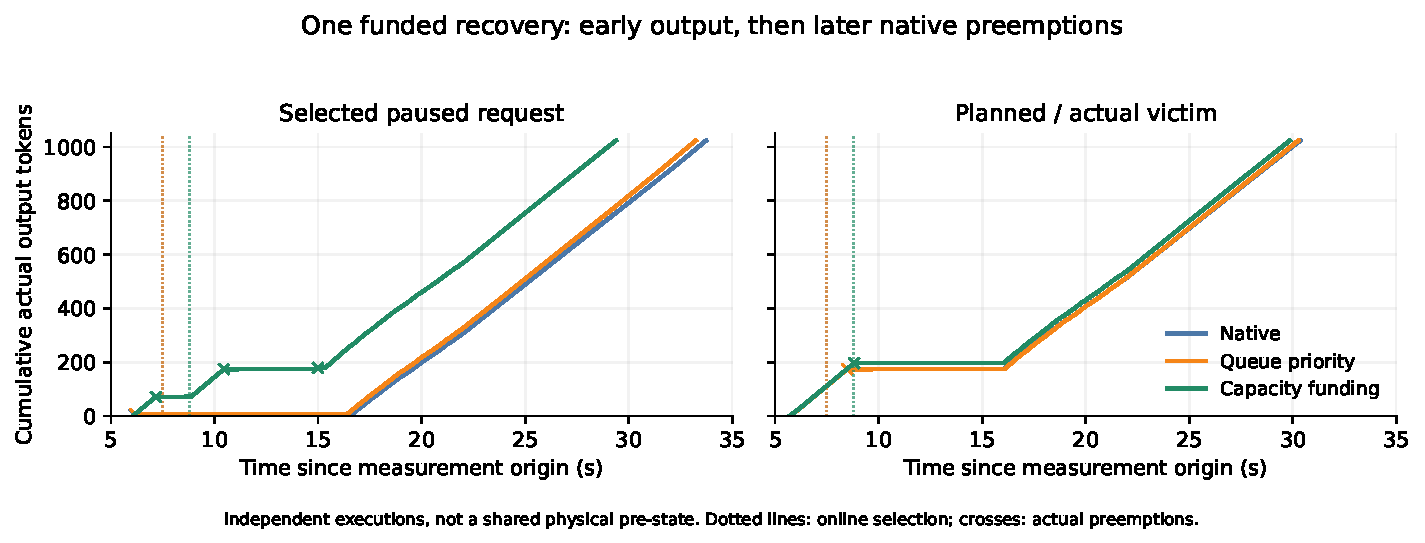
\includegraphics[width=\linewidth]{figures/oldest_admission_r03_progress.pdf}
\caption{R03 output trajectories for the selected paused request and planned or actual victim. Each arm has its own physical pre-state; dotted lines mark online selections and crosses mark native preemptions. The funded target outputs promptly but is preempted twice more after its $Q=1$ release.}
\label{fig:oldestadmissionprogress}
\end{figure}

\subsection{Repeated Oldest-Paused Admission}
An initial R01 launch stopped at the private-cache disk reserve before any cell. R02 reused the three frozen, unrun packages and the same 1.25-GiB reserve, inputs, rules, order, and scientific criteria after consolidating byte-identical payloads \cite{oldestrepeatplan}. The repeated rule keeps the one-second observed-output age gate, permits one active episode at a time, and never retries a canceled pause. In one already-seen 128-request block, every arm completes with native full saving. Queue-fund records 58 episodes involving 21 distinct target sources: 57 actual native victim preemptions and one direct resume, with no cancellations. Every $Q=1$ protection lifecycle closes and every displaced victim completes; all twenty predeclared checks pass \cite{oldestrepeat}. After the protected first output, 48/58 target episodes undergo later native preemption after a median 18 additional outputs and 0.2883 seconds. All 57 forced victims later output and complete; their preemption-to-next-output median/maximum are 1.1098/1.8455 seconds, and 46 later become funded targets, yielding overlapping absolute pauses rather than independent replicates or causal incremental costs \cite{oldestrepeatfollowup}. Table~\ref{tab:oldestrepeat} shows a funded p95 request-maximum gap of 1.552 seconds versus 7.939/9.582 for native/queue-only, within the fixed 97\% output-rate and 105\% mean-flow budgets. The cohort maximum falls to 2.188 seconds, but total native preemptions rise from 46/48 to 103, including 57 forced actions. Relative to native, 57 individual maximum gaps improve and 71 worsen; the median increases from 0.04156 to 0.05599 seconds. Among the 71 worsened requests, the median increase is 4.35 ms, but seven exceed one second; these cross-arm differences are descriptive rather than per-request causal costs \cite{oldestrepeatgaps}. Figure~\ref{fig:oldestrepeatgapecdf} shows the full request distribution. Funded goodput improves/worsens at 14/6 fixed points against each control. Native/queue-only/fund output totals are 127,401/128,154/127,286, with 4/3/4 natural stops; output sequences differ for 59/66/54 requests and stop identities for 3/4/1 across queue-only versus native, fund versus native, and fund versus queue-only. These serial trajectories are one exploratory simple-policy pilot, not equal-work acceleration, stable or fresh-input confirmation, or an independent method. Strong ordinary-backfill and closest-prior controls remain unrun for this rule \cite{cacheopt,uniboost}.

\begin{table}[h]
\centering\footnotesize
\caption{Repeated oldest-paused pilot on one already-seen block (128 completed requests per arm). P95 is across requests' maximum output gaps; all twenty prespecified checks pass in this block.}
\label{tab:oldestrepeat}
\begin{tabular}{lrrrrrr}
\toprule
Arm & Rate (tokens/s) & Mean flow (s) & P95 gap (s) & Max gap (s) & Preemptions & Forced \\
\midrule
Native & 1,507.070 & 37.055 & 7.939 & 12.066 & 46 & 0 \\
Queue only & 1,507.384 & 37.591 & 9.582 & 12.883 & 48 & 0 \\
Queue fund & 1,497.006 & 37.487 & 1.552 & 2.188 & 103 & 57 \\
\bottomrule
\end{tabular}
\end{table}

\begin{figure}[h]
\centering
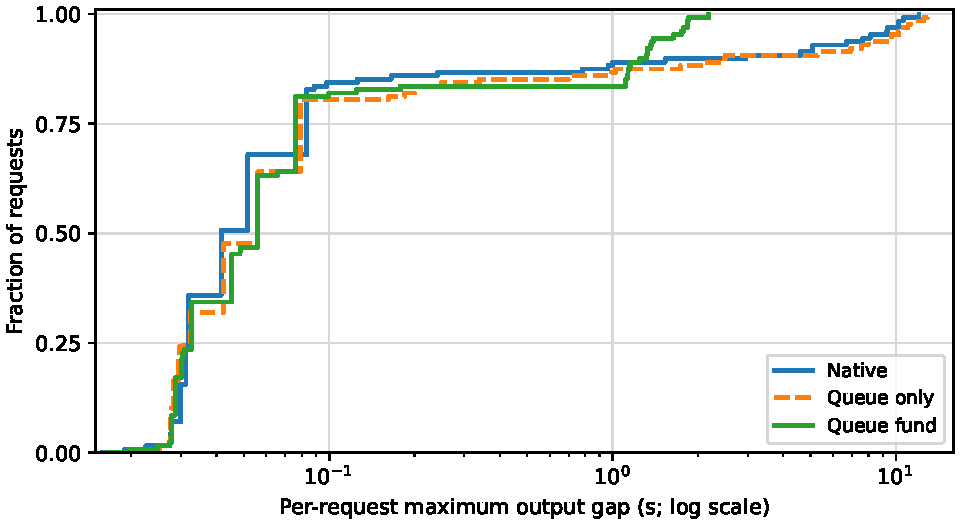
\includegraphics[width=.89\linewidth]{figures/oldest_repeat_r02_gap_ecdf.pdf}
\caption{ECDF of the maximum returned-output gap for all 128 requests in each arm of the one already-seen block. Each request has equal weight; the horizontal axis is logarithmic. Arms follow separate, independently evolving physical trajectories.}
\label{fig:oldestrepeatgapecdf}
\end{figure}

\pagebreak
\section{Related Work}
LTR studies waiting-based priority and a service quantum; our adapter transfers only these components into this native-offload setting \cite{ltr,related}. Andes jointly selects a served set under batch and KV constraints, then checks whether admission benefits exceed preemption costs to all ongoing requests \cite{andes,related}. Our capacity-qualified-victim reference fixes the recovery target and filters a single victim by current blocks; it does not implement Andes' joint QoE or peer-cost model. UniBoost includes protection tied to useful decode service and tests KV needs for upcoming work \cite{uniboost,related}. TokenFlow accounts for memory, I/O, and recomputation when organizing serving work \cite{tokenflow,related}. These published mechanisms already cover much of the apparent design space. The source comparison is a literature boundary, not an implementation-equivalence claim: we have not executed those complete systems in this environment. Classical backfilling already uses later fitting jobs to occupy otherwise idle resources after protecting progress for earlier work \cite{backfill}. Our primary-output event differs from reserving a future start time, but this does not establish a new scheduling primitive or a no-delay guarantee. A fit check, fixed quantum, reservation recheck, or bounded backfill alone cannot support novelty.

BidKV is a close public victim-selection implementation: its default score is computed tokens divided by a disruption estimate using output-to-cap progress and cumulative preemptions. Its request state is not reset at native readmission, and its numerator is computed tokens rather than measured physical KV pages. Both designs nevertheless use progress and memory-related signals for pressure-triggered victim choice. An exact-formula difference alone does not establish novelty; a constrained-score transplant must be labeled as an adaptation, not a complete BidKV reproduction \cite{bidkvcode}.

\section{Limitations and Open Work}
Each performance block ran once in sequence on one GPU. We have no variance estimate, randomized ordering beyond the specified reversal, sustained-arrival result, production SLO, or output-quality assessment. Natural generation changed token sequences and sometimes stop reasons across arms; rate and flow differences cannot be read as equal-work acceleration. The host-output timestamps do not separate device generation, transfer, queueing, and client delivery. Across the earlier eight cells, printed transfer counters cover only seven isolated complete intervals per cell after the first print, reset at each print, and omit boundary work and preceding stream waits; their CUDA time is not a request-visible stall measure \cite{printedtransfers}. The Q1/Q10 pair and yield triplet have the same printed-interval limitation \cite{capacityqtransfers,yieldtransfers}. Memory limits and nominal KV sizes are fixed, but a process-tree peak and independent KV tensor-value equivalence were not established. H128 was seen before the G64 parameter freeze, and no untouched input has confirmed a method claim.

The fit-first experiment confirms native alternative-target actions, but does not establish a method benefit. The longest-gap request was bypassed 20 times. A separate reconstruction of the earlier complete H1 diagnostic found an alternative eligible, sufficiently funded victim in all 511 funding-rejected preparation states. The capacity filter produced actual funded recovery actions in two ordered blocks, but their complete-service results disagree and fail the joint criterion. This filter is a simple baseline correction, not an independent algorithmic contribution. The two same-policy A/A pairs each show divergent natural trajectories; two single pairs cannot establish a variance bound, prove a cache mechanism, or correct all policy comparisons. The first five seconds also differ in the warm pair, and cache file modification records do not imply zero compilation. We stop expanding the A/A matrix. The resource-qualified Q1/Q10 pilot obtained real ten-output actions but failed its rate and gap conditions. The unchanged-Q10 sparse diagnostic identified real waiting-gate exclusions with numerical headroom; the conditional yield triplet then confirmed native admission and subsequent output, but failed the complete-service tail criterion against Q1 and plain Q10. Neither the fit gate nor early release is an independent method contribution. Any eventual method claim needs a prespecified difference from strong simple baselines, complete-request benefit under a common budget, and confirmation matching the intended scope. The present single new-input episode addresses a narrow simple-baseline tradeoff, not the independent-method requirement.

\section{Conclusion}
Under these fixed per-block configurations, the calibrated LTR-style component did not improve the eager reference's worst gap within the H128 transfer budget. Commit-time direct admission was observable, yet its two ordered performance pairs did not jointly improve the preset gap objective. Fit-first illustrates that average service and median gaps can improve while a few requests incur much longer pauses. The capacity-qualified victim baseline improved the first ordered block but failed the joint criterion after the reverse-order block; two identical-policy pairs also showed trajectory differences under their respective conditions. Ten-output protection and qualified early release produced observed native actions, yet both failed their exploratory complete-service gap criteria. The bounded post-primary-output follow-up passed the same gap and cost conditions in two ordered seen-input blocks, but harmed individual requests and increased total preemptions. One frozen new-input triplet also passed the original criteria, with 18 observed follow-ups and a 22.754\% smaller maximum gap than Q1; native full saving retained better mean completion at a substantially longer gap tail. The subsequent ordinary-backfill control also met the declared goal and exceeded primary-first goodput at all twenty fixed points within its own block; primary-first retained only a lower cohort maximum among the gap metrics. The native full-save ordinary-only pair further confirms 23 real recoveries without proactive rotations, but fails both efficiency conditions despite improving the gap tail. A subsequent implementation-only pair reduced per-call \texttt{begin} CPU by 84.59\%, while retaining mixed request-level consequences and no maximum-gap improvement. Without timers, a further optimized-ordinary/native pair passes the original joint criteria and improves all twenty fixed goodput rates, while preserving seventeen individual gap regressions and changed natural outputs. This is a seen-input implementation qualification. A further native allocation-failure victim triplet obtains a smaller worst gap with residence density than with tail or original-arrival selection, within the predefined efficiency budget, while worsening the arrival control's p90/p95 gaps and most individual completion times. The direct action is executable. A separate factor ablation gives the complete score a lower maximum gap, higher actual output rate, and lower mean flow than either simpler score, while preserving mixed request-level effects. Both frozen new-input blocks then fail the original tail-relative maximum-gap condition: density versus tail is 10.071 versus 8.391 seconds and 9.034 versus 8.357 seconds, respectively. A guarded continuation admits successor work after 29 actual self-preemptions but has a 10.750-second maximum gap, worse than both original-break controls in its one ordered triplet. In another seen-input block, a restricted adaptation of the official BidKV score passes the separate score-baseline criterion, and its eight guarded continuations pass their service criterion; neither is a full BidKV reproduction or new-input confirmation. A current-request guard subsequently passes its seen-input pilot but fails both frozen new-input blocks, so we stop expanding that rule. These observations strengthen the simple baseline and leave the paper's central independent-method contribution unresolved. This document is a research working draft, not a submission-ready result.

\begin{thebibliography}{10}
\bibitem{argument} Internal research argument. \nolinkurl{PAPER_ARGUMENT.md}, 1 October 2026.
\bibitem{related} Internal literature recovery notes. \nolinkurl{RELATED_WORK_RECOVERY_20260914.md}, 14 September 2026.
\bibitem{liveness} Internal G64 native liveness result. \nolinkurl{A_G64_LIVENESS_RESULT_20260930.md}, 30 September 2026.
\bibitem{calibration} Internal corrected G64 calibration. \nolinkurl{A_G64_GUARDED_CALIBRATION_20260930.md}, 30 September 2026.
\bibitem{htransfer} Internal H128 guarded transfer result. \nolinkurl{A_H128_GUARDED_TRANSFER_RESULT_20260930.md}, 30 September 2026.
\bibitem{h1qual} Internal H1 native direct-action qualification. \nolinkurl{A_H1_NATIVE_DIRECT_QUALIFICATION_RESULT_20261001.md}, 1 October 2026.
\bibitem{h1pairs} Internal H1 paired performance result. \nolinkurl{A_H1_PERFORMANCE_PAIRED_RESULT_R01_20261001.md}, 1 October 2026.
\bibitem{capacitypair} Internal first capacity-qualified victim paired result. \nolinkurl{A_CAPACITY_VICTIM_PAIR_RESULT_R01_20261001.json}, 1 October 2026.
\bibitem{capacitypairb2} Internal reverse-order capacity-qualified victim paired result. \nolinkurl{A_CAPACITY_VICTIM_PAIR_B2_RESULT_R01_20261001.json}, 1 October 2026.
\bibitem{capacityaa} Internal capacity-qualified victim same-policy A/A result. \nolinkurl{A_CAPACITY_IDENTICAL_PAIR_RESULT_R01_20261001.json}, 1 October 2026.
\bibitem{capacityphases} Internal same-policy A/A phase description. \nolinkurl{A_CAPACITY_IDENTICAL_PHASES_R01_20261001.json}, 1 October 2026.
\bibitem{capacitycache} Internal same-policy A/A cache file phase inventory. \nolinkurl{A_CAPACITY_IDENTICAL_CACHE_PHASES_R01_20261001.json}, 1 October 2026.
\bibitem{warmcapacityaa} Internal warm-cache same-policy A/A result. \nolinkurl{A_CAPACITY_WARM_IDENTICAL_PAIR_RESULT_R02_20261001.json}, 1 October 2026.
\bibitem{warmcapacityphases} Internal warm-cache same-policy phase description. \nolinkurl{A_CAPACITY_WARM_IDENTICAL_PHASES_R02_20261001.json}, 1 October 2026.
\bibitem{warmcapacitycache} Internal warm-cache seed receipt and two cell write summaries. \nolinkurl{moe-a-capacity-warm-identical-session-r02-20261001/}, 1 October 2026.
\bibitem{capacityq} Internal Q1/Q10 capacity-qualified protection pilot. \nolinkurl{A_CAPACITY_PROTECTION_PAIR_RESULT_R03_20261001.md}, 1 October 2026.
\bibitem{capacityqpeer} Internal complete-request target/peer description. \nolinkurl{A_CAPACITY_PROTECTION_TARGET_PEER_R03_20261001.json}, 1 October 2026.
\bibitem{capacityqexposure} Internal Q1/Q10 early-trajectory and extension exposure description. \nolinkurl{A_CAPACITY_PROTECTION_EXPOSURE_R03_20261001.json}, 1 October 2026.
\bibitem{capacityqtransfers} Internal Q1/Q10 printed transfer interval description. \nolinkurl{A_CAPACITY_PROTECTION_PRINTED_TRANSFERS_R03_20261001.json}, 1 October 2026.
\bibitem{printedtransfers} Internal printed transfer interval summary. \nolinkurl{A_PRINTED_TRANSFER_INTERVALS_R01_20261001.json}, 1 October 2026.
\bibitem{ltr} LTR, version 1, Section 4.3. \url{https://arxiv.org/html/2408.15792v1#S4.SS3}.
\bibitem{andes} Andes, version 2, Section 4. \url{https://arxiv.org/html/2404.16283v2#S4}.
\bibitem{uniboost} UniBoost, version 1, Section 3.3. \url{https://arxiv.org/html/2606.18431v1#S3.SS3}.
\bibitem{tokenflow} TokenFlow, version 1, Section 4. \url{https://arxiv.org/html/2510.02758v1#S4}.
\bibitem{protectionscope} Internal unchanged-Q10 native protection-scope observation. \nolinkurl{A_PROTECTION_SCOPE_DIAG_RESULT_R01_20261001.md}, 1 October 2026.
\bibitem{yieldtriplet} Internal Q1/conditional-yield/plain-Q10 native triplet. \nolinkurl{A_PROTECTION_YIELD_TRIPLET_RESULT_R01_20261001.md}, 1 October 2026.
\bibitem{yieldtransfers} Internal triplet printed transfer intervals. \nolinkurl{A_PROTECTION_YIELD_PRINTED_TRANSFERS_R01_20261001.json}, 1 October 2026.
\bibitem{yieldpeer} Internal triplet target, peer, and longest-pause follow-up. \nolinkurl{A_PROTECTION_YIELD_TRIPLET_TARGET_PEER_R01_20261001.json}, 1 October 2026.
\bibitem{spareopportunity} Internal first-output spare-capacity reconstruction. \nolinkurl{A_SPARE_FOLLOWUP_OPPORTUNITY_R01_20261001.json}, 1 October 2026.
\bibitem{sparepair} Internal native spare-follow-up off/on pair. \nolinkurl{A_SPARE_FOLLOWUP_PAIR_RESULT_R01_20261001.md}, 1 October 2026.
\bibitem{sparepeer} Internal spare-follow-up actor costs and longest-gap description. \nolinkurl{A_SPARE_FOLLOWUP_TARGET_PEER_R01_20261001.json}, 1 October 2026.
\bibitem{sparetransfers} Internal spare-follow-up printed transfer intervals. \nolinkurl{A_SPARE_FOLLOWUP_PRINTED_TRANSFERS_R01_20261001.json}, 1 October 2026.
\bibitem{sparetwopairs} Internal two-block spare-follow-up result. \nolinkurl{A_SPARE_FOLLOWUP_TWO_PAIRS_RESULT_R01_20261001.md}, 1 October 2026.
\bibitem{sparepeerr02} Internal reverse-block actor costs. \nolinkurl{A_SPARE_FOLLOWUP_TARGET_PEER_R02_20261001.json}, 1 October 2026.
\bibitem{sparefreshpeer} Internal frozen new-input actor costs and gap localization. \nolinkurl{A_SPARE_FOLLOWUP_FRESH_TARGET_PEER_R01_20261001.json}, 1 October 2026.
\bibitem{sparefreshtransfers} Internal frozen new-input printed transfer intervals. \nolinkurl{A_SPARE_FOLLOWUP_FRESH_PRINTED_TRANSFERS_R01_20261001.json}, 1 October 2026.
\bibitem{sparefresh} Internal frozen new-input three-arm result. \nolinkurl{A_SPARE_FOLLOWUP_FRESH_RESULT_R01_20261001.json}, 1 October 2026.
\bibitem{nativeonly} A research artifacts. \emph{Native full-save ordinary-only pair}. \path{A_NATIVE_BACKFILL_ONLY_PAIR_RESULT_R01_20261001.json}, 2026.
\bibitem{nativeonlypeer} A research artifacts. \emph{Native full-save ordinary-only target and peer trajectories}. \path{A_NATIVE_BACKFILL_ONLY_TARGET_PEER_R01_20261001.json}, 2026.
\bibitem{nativeonlytransfers} A research artifacts. \emph{Native full-save pair printed transfer intervals}. \path{A_NATIVE_BACKFILL_ONLY_PRINTED_TRANSFERS_R01_20261001.json}, 2026.
\bibitem{nativeonlycpu} A research artifacts. \emph{Native full-save ordinary-only adapter CPU diagnostic}. \path{A_NATIVE_BACKFILL_CPU_DIAG_RESULT_R01_20261001.json}, 2026.
\bibitem{waiteractors} A research artifacts. \emph{Ordinary backfill target and peer consequences}. \path{A_WAITER_BACKFILL_TARGET_PEER_R01_20261001.json}, 2026.
\bibitem{waitercontrol} Internal ordinary-backfill strong-control triplet. \nolinkurl{A_WAITER_BACKFILL_TRIPLET_RESULT_R01_20261001.json}, 1 October 2026.
\bibitem{backfill} E. Shmueli and D. G. Feitelson. Backfilling with Lookahead to Optimize the Packing of Parallel Jobs. 2005. \url{https://research.ibm.com/publications/backfilling-with-lookahead-to-optimize-the-packing-of-parallel-jobs}.
\bibitem{nativelazy} A research artifacts. \emph{Original versus on-demand running-view construction, timed native full-save pair}. \path{A_NATIVE_BACKFILL_LAZY_PAIR_RESULT_R01_20261002.json}, 2 October 2026.
\bibitem{nativelazyperf} A research artifacts. \emph{Untimed optimized ordinary/native full-save qualification}. \path{A_NATIVE_BACKFILL_LAZY_PERF_PAIR_RESULT_R01_20261002.json}, 2 October 2026.
\bibitem{nativelazyperfcost} A research artifacts. \emph{Observed printed transfer counters for the untimed qualification}. \path{A_NATIVE_BACKFILL_LAZY_PERF_PRINTED_TRANSFERS_R01_20261002.json}, 2 October 2026.
\bibitem{nativelazyperfpeer} A research artifacts. \emph{Untimed optimized ordinary/native target and peer trajectories}. \path{A_NATIVE_BACKFILL_LAZY_PERF_TARGET_PEER_R01_20261002.json}, 2 October 2026.
\bibitem{residencyshort} A research artifacts. \emph{Ordinary recovery short-service episodes}. \path{A_NATIVE_BACKFILL_LAZY_SHORT_SERVICE_R01_20261002.json}, 2 October 2026.
\bibitem{residencyvictim} A research artifacts. \emph{Native allocation-failure victim triplet}. \path{A_NATIVE_RESIDENCY_VICTIM_TRIPLET_RESULT_R01_20261002.json}, 2 October 2026.
\bibitem{residencycost} A research artifacts. \emph{Victim triplet observed printed transfer counters}. \path{A_NATIVE_RESIDENCY_VICTIM_PRINTED_TRANSFERS_R01_20261002.json}, 2 October 2026.
\bibitem{residencyepochs} A research artifacts. \emph{Initial and restored victim residence epochs}. \path{A_NATIVE_RESIDENCY_VICTIM_EPOCH_FOLLOWUP_R01_20261002.json}, 2 October 2026.
\bibitem{residencyablation} A research artifacts. \emph{Residence reset and KV normalization ablation}. \path{A_NATIVE_RESIDENCY_ABLATION_PRIMARY_TRIPLET_RESULT_R01_20261002.json}, 2 October 2026.
\bibitem{residencyfreshb1} A research artifacts. \emph{First frozen new-input victim-selection block}. \path{A_NATIVE_RESIDENCY_FRESH_B1_RESULT_R01_20261002.json}, 2 October 2026.
\bibitem{residencyfreshb2} A research artifacts. \emph{Reverse-order frozen new-input victim-selection block}. \path{A_NATIVE_RESIDENCY_FRESH_B2_RESULT_R01_20261002.json}, 2 October 2026.
\bibitem{residencyfreshtwo} A research artifacts. \emph{Two-block frozen new-input victim-selection result}. \path{A_NATIVE_RESIDENCY_FRESH_TWO_BLOCKS_RESULT_R01_20261002.json}, 2 October 2026.
\bibitem{residencyfreshchain} A research artifacts. \emph{Observed first-block maximum-gap chain}. \path{A_NATIVE_RESIDENCY_FRESH_B1_MAX_GAP_CHAIN_R01_20261002.json}, 2 October 2026.
\bibitem{residencyselfsuffix} A research artifacts. \emph{Self-preemption with remaining running successors}. \path{A_NATIVE_RESIDENCY_SELF_PREEMPT_SUFFIX_R01_20261002.json}, 2 October 2026.
\bibitem{residencycontinue} A research artifacts. \emph{Guarded self-preemption continuation triplet}. \path{A_NATIVE_SELF_PREEMPT_CONTINUE_TRIPLET_RESULT_R01_20261002.json}, 2 October 2026.
\bibitem{bidkvresult} A research artifacts. \emph{Pinned BidKV-score adaptation and guarded continuation triplet}. \path{A_NATIVE_BIDKV_SCORE_TRIPLET_RESULT_R01_20261002.json}, 2 October 2026.
\bibitem{bidkvguardresult} A research artifacts. \emph{Current-request guard on the pinned-score adaptation}. \path{A_NATIVE_CURRENT_GUARD_TRIPLET_RESULT_R02_20261002.json}, 2 October 2026.
\bibitem{bidkvcode} BidKV maintainers. \emph{Utility victim selector}, commit \texttt{5ee8025}. \url{https://github.com/vLLM-HUST/vllm-ascend-hust-bidkv/blob/5ee80256d263d58b1e512d9d436d47e9bac564ba/vllm_ascend_bidkv/selector.py}, accessed 2 October 2026.
\bibitem{guardfreshtwo} A research artifacts. \emph{Frozen current-request guard, both opposite-order blocks}. \path{A_NATIVE_CURRENT_GUARD_FRESH_TWO_BLOCKS_RESULT_R02_20261002.json}, 2 October 2026.
\bibitem{guardfreshchain} A research artifacts. \emph{First fresh block's observed longest-gap chain}. \path{A_NATIVE_CURRENT_GUARD_FRESH_B1_FAILURE_CHAIN_R02_20261002.json}, 2 October 2026.
\bibitem{guardfreshchainb2} A research artifacts. \emph{Second fresh block's repeated-preemption and longest-gap chain}. \path{A_NATIVE_CURRENT_GUARD_FRESH_B2_FAILURE_CHAIN_R02_20261002.json}, 2 October 2026.
\bibitem{bidkvfullrunning} A research artifacts. \emph{Full-running pinned BidKV-score baseline qualification triplet}. \path{A_NATIVE_BIDKV_FULL_RUNNING_TRIPLET_RESULT_R01_20261002.json}, 2 October 2026.
\bibitem{completiondeferral} A research artifacts. \emph{Native completion-funded prefix deferral triplet}. \path{A_NATIVE_COMPLETION_DEFERRAL_TRIPLET_RESULT_R01_20261002.json}, 2 October 2026.
\bibitem{completiongroups} A research artifacts. \emph{Grouped observed completion-deferral events}. \path{A_NATIVE_COMPLETION_DEFERRAL_GROUPS_R01_20261002.json}, 2 October 2026.
\bibitem{cacheopt} H. Shen, T. Sen, and M. Tanaka. \emph{Mitigating KV Cache Competition to Enhance User Experience in LLM Inference}. arXiv:2503.13773v2, 2025. \url{https://arxiv.org/html/2503.13773v2}.
\bibitem{victimsizer02} A research artifacts. \emph{Native physical-size victim triplet}. \path{A_NATIVE_VICTIM_SIZE_TRIPLET_RESULT_R02_20261002.json}, 2 October 2026.
\bibitem{victimsizeplan} A research artifacts. \emph{Resource-only retry and unchanged physical-size victim protocol}. \path{NATIVE_VICTIM_SIZE_TRIPLET_PLAN_R02_20261002.json}, 2 October 2026.
\bibitem{oldestadmission} A research artifacts. \emph{One-shot oldest-paused native admission triplet}. \path{A_NATIVE_OLDEST_ADMISSION_TRIPLET_RESULT_R01_20261002.json}, 2 October 2026.
\bibitem{oldestadmissionr03} A research artifacts. \emph{Gate-corrected one-shot oldest-paused native admission triplet}. \path{A_NATIVE_OLDEST_ADMISSION_TRIPLET_RESULT_R03_20261002.json}, 2 October 2026.
\bibitem{oldestadmissionplanr03} A research artifacts. \emph{R02 resource abort and R03 unchanged one-shot protocol}. \path{NATIVE_OLDEST_ADMISSION_TRIPLET_PLAN_R03_20261002.json}, 2 October 2026.
\bibitem{oldestadmissionfollowup} A research artifacts. \emph{R03 oldest-admission target and victim action follow-up}. \path{A_NATIVE_OLDEST_ADMISSION_ACTION_FOLLOWUP_R03_20261002.json}, 2 October 2026.
\bibitem{oldestrepeat} A research artifacts. \emph{Repeated oldest-paused native admission triplet}. \path{A_NATIVE_OLDEST_REPEAT_TRIPLET_RESULT_R02_20261002.json}, 2 October 2026.
\bibitem{oldestrepeatplan} A research artifacts. \emph{R01 resource abort and unchanged repeated-policy protocol}. \path{NATIVE_OLDEST_REPEAT_TRIPLET_PLAN_R02_20261002.json}, 2 October 2026.
\bibitem{oldestrepeatfollowup} A research artifacts. \emph{Repeated oldest-paused target and victim action follow-up}. \path{A_NATIVE_OLDEST_REPEAT_ACTION_FOLLOWUP_R02_20261002.json}, 2 October 2026.
\bibitem{oldestrepeatgaps} A research artifacts. \emph{Repeated oldest-paused request-gap segments}. \path{A_NATIVE_OLDEST_REPEAT_GAP_SEGMENTS_R02_20261002.json}, 2 October 2026.
\end{thebibliography}
\end{document}
